%%%%%%%%%%%%%%%%%%%%%%%%%%%%%%%%%%%%%%%%%%%%%%%%%%%%%%%%%%%%%%%%%%%%%%%%
%% Customizações do abnTeX2 (http://abnTeX2.googlecode.com)           %%
%% para a Universidade Estadual do Ceara - UECE                       %%
%%                                                                    %%
%% This work may be distributed and/or modified under the             %% 
%% conditions of the LaTeX Project Public License, either version 1.3 %%
%% of this license or (at your option) any later version.             %%
%% The latest version of this license is in                           %%
%%   http://www.latex-project.org/lppl.txt                            %%
%% and version 1.3 or later is part of all distributions of LaTeX     %%
%% version 2005/12/01 or later.                                       %%
%%                                                                    %%
%% This work has the LPPL maintenance status `maintained'.            %%
%%                                                                    %%
%% The Current Maintainer of this work is Thiago Nascimento           %%
%%                                                                    %%
%% Project available on: https://github.com/thiagodnf/uecetex2        %%
%%                                                                    %%
%% Further information about abnTeX2                                  %%
%% are available on http://abntex2.googlecode.com/                    %%
%%                                                                    %%
%%%%%%%%%%%%%%%%%%%%%%%%%%%%%%%%%%%%%%%%%%%%%%%%%%%%%%%%%%%%%%%%%%%%%%%%
\documentclass[        
    a4paper,          % Tamanho da folha A4
    12pt,             % Tamanho da fonte 12pt
    chapter=TITLE,    % Todos os capitulos devem ter caixa alta
    section=TITLE,    % Todas as secoes devem ter caixa alta
    oneside,          % Usada para impressao em apenas uma face do papel
    english,          % Hifenizacoes em ingles
    spanish,          % Hifenizacoes em espanhol
    brazil            % Ultimo idioma eh o idioma padrao do documento
]{abntex2}

% Importações de pacotes
\usepackage[utf8]{inputenc}                         % Acentuação direta
\usepackage[T1]{fontenc}                            % Codificação da fonte em 8 bits


%%%%%%%%%%%%%%%%%%%%%%%%%%%%%%%%%%%%%%%%%%%%%%%%%%%%%%%%%%%%%%%%%%%%%%%%
%% Customizações do abnTeX2 (http://abnTeX2.googlecode.com)           %%
%% para a Universidade Estadual do Ceara - UECE                       %%
%%                                                                    %%
%% This work may be distributed and/or modified under the             %% 
%% conditions of the LaTeX Project Public License, either version 1.3 %%
%% of this license or (at your option) any later version.             %%
%% The latest version of this license is in                           %%
%%   http://www.latex-project.org/lppl.txt                            %%
%% and version 1.3 or later is part of all distributions of LaTeX     %%
%% version 2005/12/01 or later.                                       %%
%%                                                                    %%
%% This work has the LPPL maintenance status `maintained'.            %%
%%                                                                    %%
%% The Current Maintainer of this work is Thiago Nascimento           %%
%%                                                                    %%
%% Project available on: https://github.com/thiagodnf/uecetex2        %%
%%                                                                    %%
%% Further information about abnTeX2                                  %%
%% are available on http://abntex2.googlecode.com/                    %%
%%                                                                    %%
%%%%%%%%%%%%%%%%%%%%%%%%%%%%%%%%%%%%%%%%%%%%%%%%%%%%%%%%%%%%%%%%%%%%%%%%

\usepackage{graphicx}                               % Inserir figuras
\usepackage{amsfonts, amssymb, amsmath}             % Fonte e símbolos matemáticos
\usepackage{booktabs}                               % Comandos para tabelas
\usepackage{verbatim}                               % Texto é interpretado como escrito no documento
\usepackage{multirow, array}                        % Múltiplas linhas e colunas em tabelas
\usepackage{indentfirst}                            % Endenta o primeiro parágrafo de cada seção.
\usepackage{listings}                               % Utilizar codigo fonte no documento
\usepackage{xcolor}
\usepackage{microtype}                              % Para melhorias de justificação?
\usepackage[portuguese,ruled,lined]{algorithm2e}    % Escrever algoritmos
\usepackage{algorithmic}                            % Criar Algoritmos  
%\usepackage{float}                                  % Utilizado para criação de floats
\usepackage{amsgen}
\usepackage{lipsum}                                 % Usar a simulação de texto Lorem Ipsum
%\usepackage{titlesec}                               % Permite alterar os títulos do documento
\usepackage{tocloft}                                % Permite alterar a formatação do Sumário
\usepackage{etoolbox}                               % Usado para alterar a fonte da Section no Sumário
\usepackage[nogroupskip,nonumberlist,acronym]{glossaries}                % Permite fazer o glossario
\usepackage{caption}                                % Altera o comportamento da tag caption
\usepackage[alf, abnt-emphasize=bf, bibjustif, recuo=0cm, abnt-etal-cite=2, abnt-etal-list=0]{abntex2cite}  % Citações padrão ABNT
%\usepackage[bottom]{footmisc}                      % Mantém as notas de rodapé sempre na mesma posição
%\usepackage{times}                                 % Usa a fonte Times
\usepackage{mathptmx}                               % Usa a fonte Times New Roman										
%\usepackage{lmodern}                               % Usa a fonte Latin Modern
%\usepackage{subfig}                                % Posicionamento de figuras
%\usepackage{scalefnt}                              % Permite redimensionar tamanho da fonte
%\usepackage{color, colortbl}                       % Comandos de cores
%\usepackage{lscape}                                % Permite páginas em modo "paisagem"
%\usepackage{ae, aecompl}                           % Fontes de alta qualidade
%\usepackage{picinpar}                              % Dispor imagens em parágrafos
%\usepackage{latexsym}                              % Símbolos matemáticos
%\usepackage{upgreek}                               % Fonte letras gregas
\usepackage{appendix}                               % Gerar o apendice no final do documento
\usepackage{paracol}                                % Criar paragrafos sem identacao
\usepackage{lib/uecetex2}		                    % Biblioteca com as normas da UECE para trabalhos academicos
\usepackage{pdfpages}                               % Incluir pdf no documento
\usepackage{amsmath}                                % Usar equacoes matematicas

% Organiza e gera a lista de abreviaturas, simbolos e glossario
\makeglossaries

% Gera o Indice do documento
\makeindex


%%%%%%%%%%%%%%%%%%%%%%%%%%%%%%%%%%%%%%%%%%%%%%%%%%%%%
%%          Configuracoes do ueceTeX2              %%
%%%%%%%%%%%%%%%%%%%%%%%%%%%%%%%%%%%%%%%%%%%%%%%%%%%%%

% Opcoes disponiveis

\trabalhoacademico{tccgraduacao}
%\trabalhoacademico{tccespecializacao}
% \trabalhoacademico{dissertacao}
%\trabalhoacademico{tese}

% Define se o trabalho eh uma qualificacao
% Coloque 'nao' para versao final do trabalho

\ehqualificacao{nao}

% Remove as bordas vermelhas e verdes do PDF gerado
% Coloque 'sim' pare remover

\removerbordasdohyperlink{sim} 

% Adiciona a cor Azul a todos os hyperlinks

\cordohyperlink{nao}

%%%%%%%%%%%%%%%%%%%%%%%%%%%%%%%%%%%%%%%%%%%%%%%%%%%%%
%%          Informação sobre a IES                 %%
%%%%%%%%%%%%%%%%%%%%%%%%%%%%%%%%%%%%%%%%%%%%%%%%%%%%%

\ies{Faculdade Bilac}
\iessigla{BILAC}
% \centro{Centro de Ciências e Tecnologia}

%%%%%%%%%%%%%%%%%%%%%%%%%%%%%%%%%%%%%%%%%%%%%%%%%%%%%
%%        Informação para TCC de Graduacao         %%
%%%%%%%%%%%%%%%%%%%%%%%%%%%%%%%%%%%%%%%%%%%%%%%%%%%%%

\graduacaoem{Ciência da Computação}
\habilitacao{bacharel} % Pode colocar tambem 'licenciada'

%%%%%%%%%%%%%%%%%%%%%%%%%%%%%%%%%%%%%%%%%%%%%%%%%%%%%
%%     Informação para TCC de Especializacao       %%
%%%%%%%%%%%%%%%%%%%%%%%%%%%%%%%%%%%%%%%%%%%%%%%%%%%%%



%%%%%%%%%%%%%%%%%%%%%%%%%%%%%%%%%%%%%%%%%%%%%%%%%%%%%
%%         Informação para Dissertacao             %%
%%%%%%%%%%%%%%%%%%%%%%%%%%%%%%%%%%%%%%%%%%%%%%%%%%%%%

% \programamestrado{Programa de Pós-Graduação em Ciência da Computação}
% \nomedomestrado{Trabalho de conclusão de curso em Ciência da Computação}
% \mestreem{Ciência da Computação}
% \areadeconcentracaomestrado{Ciência da Computação}

%%%%%%%%%%%%%%%%%%%%%%%%%%%%%%%%%%%%%%%%%%%%%%%%%%%%%
%%               Informação para Tese              %%
%%%%%%%%%%%%%%%%%%%%%%%%%%%%%%%%%%%%%%%%%%%%%%%%%%%%%



%%%%%%%%%%%%%%%%%%%%%%%%%%%%%%%%%%%%%%%%%%%%%%
%%  Informação relacionadas ao trabalho     %%
%%%%%%%%%%%%%%%%%%%%%%%%%%%%%%%%%%%%%%%%%%%%%%

\autor{\textnormal{Daniel Varjão} Chaves \\ \textnormal{Rômulo Lima de} Oliveira  \\ \textnormal{Talita Andressa Martins} Pinto }
\titulo{Caapora RPG}
\data{2015}
\local{São José do Campos -- São Paulo}

% Exemplo: \dataaprovacao{01 de Janeiro de 2012}
\dataaprovacao{}

%%%%%%%%%%%%%%%%%%%%%%%%%%%%%%%%%%%%%%%%%%%%%
%%     Informação sobre o Orientador       %%
%%%%%%%%%%%%%%%%%%%%%%%%%%%%%%%%%%%%%%%%%%%%%

\orientador{Prof. Msc Marcos Flávio de Souza Reis}
 
\orientadorcentro{Faculdade Bilac}
\orientadorfeminino{nao} % Coloque 'sim' se for do sexo feminino

%%%%%%%%%%%%%%%%%%%%%%%%%%%%%%%%%%%%%%%%%%%%%
%%      Informação sobre o Co-orientador   %%
%%%%%%%%%%%%%%%%%%%%%%%%%%%%%%%%%%%%%%%%%%%%%

% Deixe o nome do coorientador em branco para remover do documento
% Coloque 'sim' se for do sexo feminino

%%%%%%%%%%%%%%%%%%%%%%%%%%%%%%%%%%%%%%%%%%%%%
%%      Informação sobre a banca           %%
%%%%%%%%%%%%%%%%%%%%%%%%%%%%%%%%%%%%%%%%%%%%%

% Atenção! Deixe o nome do membro da banca para remover da folha de aprovacao

% Exemplo de uso:
% \membrodabancadois{Prof. Dr. Fulano de Tal}
% \membrodabancadoisies{Universidade Estadual do Ceará - UECE}
\membrodabancadois{Prof. Me. Gerson Penha Neto}

\membrodabancadoisies{Faculdade Bilac}

\membrodabancatres{Prof. Valentino D'Ambrosi Junior}

\membrodabancatresies{Faculdade Bilac}



\begin{document}

	% Elementos pré-textuais
	\imprimircapa
    \imprimirfolhaderosto{}
	\imprimirfichacatalografica{elementos-pre-textuais/ficha-catalografica}
	\imprimirfolhadeaprovacao
	\imprimirdedicatoria{elementos-pre-textuais/dedicatoria}
	\imprimiragradecimentos{elementos-pre-textuais/agradecimentos}
	\imprimirepigrafe{elementos-pre-textuais/epigrafe}
	\imprimirresumo{elementos-pre-textuais/resumo}
	\imprimirabstract{elementos-pre-textuais/abstract}
	\imprimirlistadeilustracoes
	\imprimirlistadetabelas
%	\imprimirlistadequadros
%	\imprimirlistadealgoritmos
%	\imprimirlistadecodigosfonte
	\imprimirlistadeabreviaturasesiglas
	\imprimirlistadesimbolos{elementos-pre-textuais/lista-de-simbolos}
	\imprimirsumario
	
	%Elementos textuais
	\textual
	\chapter{Introdução}
\label{cap:introducao}
 
 
Em 1958 surgia o primeiro jogo eletrônico com o nome de "Tênis para dois", criado pelo físico William Higinbotham.O jogo era processado por um computador analógico e exibido em um osciloscópio.
\cite{mass}


Em 1961 um grupo de estudantes do MIT desenvolveram o jogo Spacewar! No jogo o objetivo era que os jogadores controlassem suas naves num ambiente escuro tentando abater o adversário. O jogo era desenvolvido num grande computador, que ocupava o espaço de uma sala inteira, o DEC PDP-1, este computador tinha como objetivo executar cálculos em geral porém apos o jogo Spacewar! o computador ficou famoso pela possibilidade de entreter outros. \cite{ram}


Foi então em 1972 que o primeiro jogo comercial foi lançado pela Atari, o Pong, ilustrado na figura 1. Era um jogo simples e intuitivo, características que o fez ser tao popular para a época. \cite{tracc} 

\begin{figure}[h!]
		\centering
		\Caption{\label{fig:exemplo-1}Jogo Pong criado pela Atari em 1972}	
		\UECEfig{}{
			\fbox{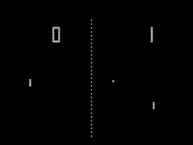
\includegraphics[width=7cm]{figuras/193px-Pong}}
		}{
			\Fonte{Wikipedia, 2015}			
		}	
	\end{figure}


Este citados foram os responsáveis pela grande diversidade e popularidade que os jogos alcançam ultimamente.

Atualmente devido a popularização da internet e dos dispositivos moveis, em destaque o uso de \textit{smartphones}no qual evidenciado na pesquisa realizada pela consultoria Nielsen 68 milhões de brasileiros utilizam \textit{smartphones} \cite{nie} 

Tendo em base a estatística da Nielsen, as palavras do diretor geral da Pontomobi, Renato Virgilli, tornam-se ainda mais expressivas diz ele: "Com o número cada vez maior de celulares, de \textit{smartphones} e de \textit{tablets} nas mãos dos usuários, cresce o interesse por aplicativos, seja para diversão ou entretenimento". \cite{vir}

Ainda de acordo com a empresa Flurry do grupo Yahoo, o uso de aplicativos cresceu em media 76\% em 2014. \cite{prox}
	
	
Os aplicativos da categoria jogos tornaram-se um passatempo global, dados comprovado na pequisa  realizada pela empresa Flurry, informando que os jogadores globais (plataforma Android) gastam em media 37 minutos por dia jogando. Desses 37 minutos, a categoria que prevalece é a de jogos casuais. \cite{flur}

Uma das vias para qual o mercado de aplicativos de jogos tem mostrado desenvolvimento eficiente é como ferramenta pedagógica.
"O aluno é totalmente ativo ao usar um aplicativo, diferente de uma TV, que ele tem uma postura mais passiva. Os envolvidos no processo passam de consumidores a produtores de conteúdo, e a ter mais autonomia e criatividade, habilidades que serão demandadas no seu futuro profissional".

Considerações essa de Tori, coordenador do Laboratório de Tecnologias Interativas da USP (Universidade de São Paulo) de que o aplicativo tem a capacidade de auxiliar o desenvolvimento de uma tarefa, e que a escola não pode viver numa realidade desconectada da do aluno.

A professora e diretora-executiva do Instituto Educadigital, Priscila Gonsales vem com o conceito de que recurso digitais e audiovisuais auxiliam a interação e visualização, aponta também que o aplicativo não substitui a metodologia tradicional e a utilização da ferramenta deva ser contextual ao conteúdo abordado. \cite{tori}

Baseando-se nos itens descritos acima: popularidade no uso de aplicativos e que este tem eficiência no uso didático, foi desenvolvido e sera apresentado neste documento o jogo digital Caapora, que tem como objetivo ensinar crianças sobre a importância da preservação da mata e ressaltar a cultura folclórica brasileira.
Aplicativo este desenvolvido para uso em  dispositivos moveis com sistema operacional Android.

\section{Motivação}
\label{cap:motivacao}

A floresta amazônica faz parte do ecossistema do mundo, é fundamental para o equilíbrio climático e é conhecida por ser o pulmão do mundo. Faz parte de 9 países dentre eles Brasil, Bolívia, Peru, Colômbia, Equador e Venezuela. E contém metade dos animais terrestres do planeta.

Apesar da extensão e de sua importância a floresta Amazônica sofre uma grande degradação causada pelo desmatamento predatório e ilegal, poluição de rios, desequilíbrio em sua fauna e flora e em vezes ocorrendo a expulsão a força de populações nativas de seus territórios.

Em uma recente pesquisa da ONG Instituto do Homem e do Meio Ambiente da Amazônia (Imazon) do Pará, o aumento do desmatamento cresceu mais de 400\% em comparação a novembro de 2013. \cite{des}

Outra grande riqueza que a Amazônia brasileira possui, é a sua grande diversidade de cultura, na parte que engloba a Amazônia brasileira (Acre, Amapá, Amazonas, Pará, Rondônia, Roraima e parte dos estados do Mato Grosso, Tocantins e Maranhão) tem-se os contos folclóricos, que segundo a carta do Folclore Brasileiro \cite{fc}, folclore é o conjunto das criações culturais de uma comunidade, baseado nas suas tradições expressas individual ou coletivamente, representativo de sua identidade social.

Em grande parte dos contos folclóricos os personagens são criaturas místicas tendo alguns deles o objetivo de proteger a floresta e as criaturas nela habitadas.


Um exemplo deste personagem é o Caipora (Caapora, em tupi, significa habitante do mato \cite{sig}), vive montado em um porco do mato e é conhecido por espantar os madeireiros com seu assobio, ajudar animais presos em armadilhas e aprontar travessuras, com o objetivo de espantar os que estão fazendo mal a mãe natureza. 

Segundo Franchini o caipora é conhecido por várias regiões do brasil, mas a sua forma física e seu método de ação varia de acordo com a região.
Na figura 2 é possível ver dois tipos diferentes em que se acreditam que o Caipora possa existir, em um ele é uma figura feminina e em outro é um menino-índio montado em um porco do mato. \cite{100}

\begin{figure}[h!]
		\centering
		\Caption{\label{fig:exemplo-4}Diversidade de formas da Caipora}	
		\UECEfig{}{
			\fbox{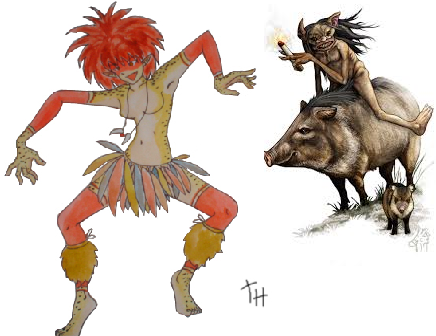
\includegraphics[width=7cm]{figuras/caipora5}}
		}{
			\Fonte{\cite{cp1}}			
		}	
	\end{figure}
	\chapter{Fundamentação Teórica}
\label{cap:fundamentacao-teorica}


\section{Os Gêneros dos Jogos}
\label{sec:os-generos-dos-jogos}

Gênero de jogo pode ser definido como uma modalidade ou tipo que permite o agrupamento de diversos jogos de acordo com suas características de jogabilidade.
Segundo Eucidio, pensar no jogo é pensar no estilo de produção que o jogo seguirá, pensar nos desafios, dificuldades e possibilidades. \cite{euc}

A plataforma dos jogos também influenciam para determinar o gênero do jogo. Em smartphones, por exemplo, os jogos tendem a ser mais casuais e rápidos. Existe uma infinidade de categorizações, abaixo encontra-se listadas alguma das mais populares. \cite{gen}

\begin{alineascomponto}
\item Jogos de Ação\\
Significa atividade, agir de acordo com  situação. O jogador tem que tomar alguma ação em tempo real, agindo rapidamente. Jogos deste gênero é o mais popular para a plataforma PC. Um exemplo de jogo de ação é o Half-Life 2, onde possui as características de ser um jogo sagaz, envolvente e com enredo, na figura 3 encontra-se a capa da Mídia digital deste jogo. \cite{gen1}
\end{alineascomponto}
\begin{figure}[h!]
		\centering
		\Caption{\label{fig:exemplo-4}Jogo Half Life 2, desenvolvido pela Valve Corporation (2004)}	
		\UECEfig{}{
			\fbox{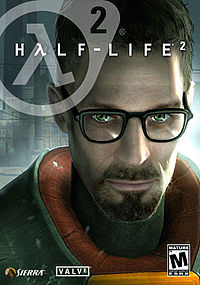
\includegraphics[width=5cm]{figuras/HalfLife}}
		}{
			\Fonte{\cite{hl}}
						
		}	
	\end{figure}
\begin{alineascomponto}
\item Jogos de Simulação\\
É a representação da realidade, são jogos que simulam situações vividas por seres humanos. A principal utilização por este gênero é para simulação de voos, tendo como objetivo o treinamento de pilotos como por exemplo o jogo FlightSimulator da Microsoft. Na figura 4 é possível ver a simulação que ocorre no jogo. \cite{gen1}
\end{alineascomponto}
\begin{figure}[h!]
		\centering
		\Caption{\label{fig:exemplo-5}Jogo Flight Simulator desenvolvido pela Microsoft (2015)}	
		\UECEfig{}{
			\fbox{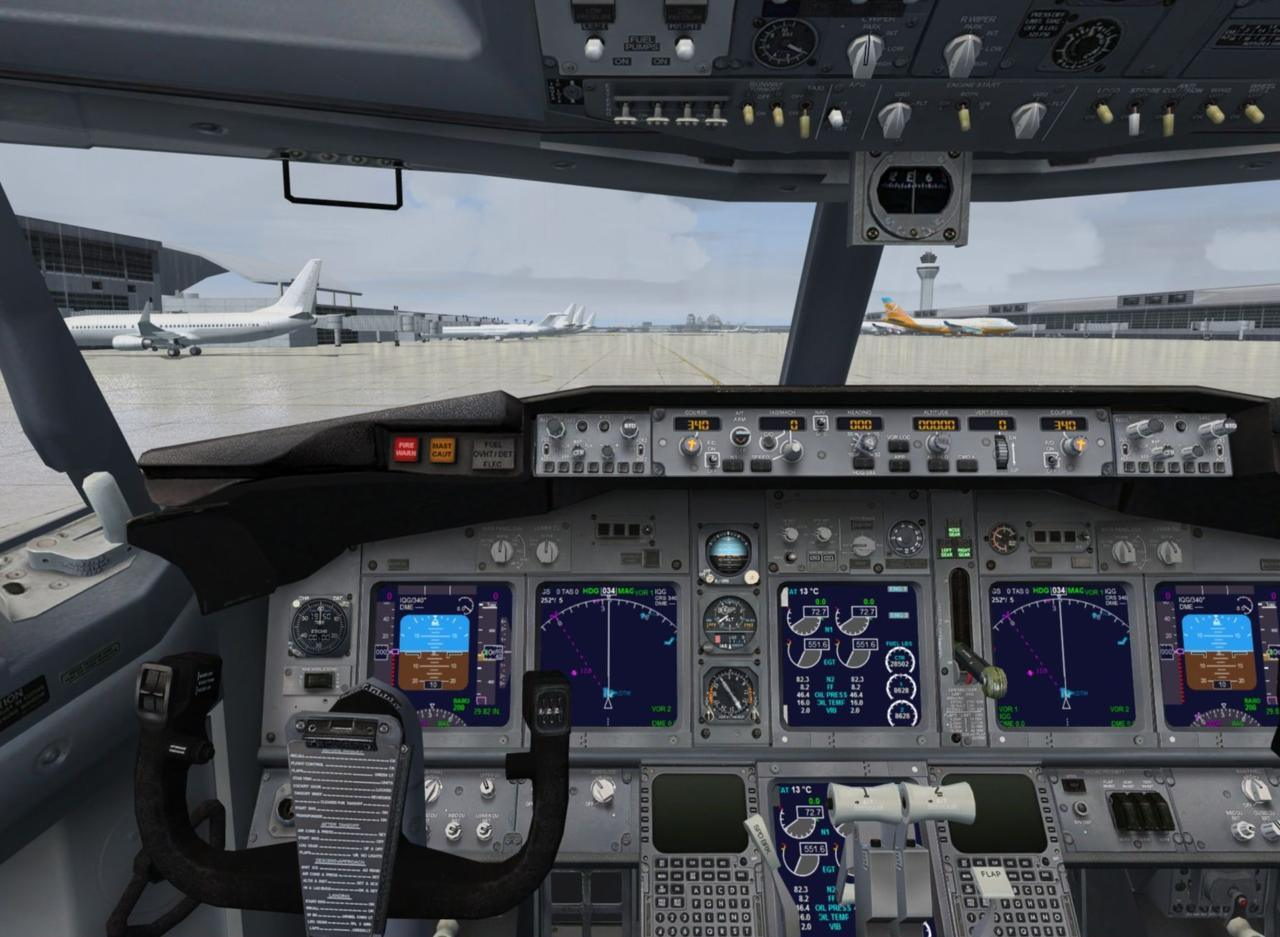
\includegraphics[width=7cm]{figuras/MFS}}
		}{
			\Fonte{\cite{fs}}			
		}	
	\end{figure}

\begin{alineascomponto}
\item Jogos de RPG\\
Tem como característica o desenvolvimento gradativo do personagem. O jogador assume o papel do personagem aonde pode haver narrativas para auxiliar no decorrer do jogo.
Um jogo muito conhecido que que utiliza deste gênero é o Final Fantasy XIII,  na figura 5 encontra-se a capa da Mídia digital deste jogo. \cite{gen1}
\end{alineascomponto}

\begin{figure}[h!]
		\centering
		\Caption{\label{fig:exemplo-6}Jogo Final Fantasy XIII desenvolvido pela Square Enix (2009)}	
		\UECEfig{}{
			\fbox{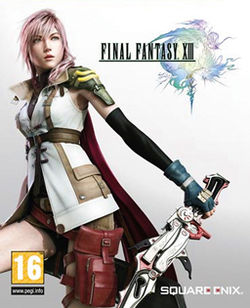
\includegraphics[width=6cm]{figuras/FF}}
		}{
			\Fonte{\cite{ff}}			
		}	
	\end{figure}
	
\begin{alineascomponto}
\item Jogos de Esportes\\
A principal característica de jogos deste gênero é o controle ocorre sobre o personagem não mecânico. Normalmente o jogo tem um esforço fısico do jogador no
mundo virtual, em alguns jogos o personagem cansa e diminui sua velocidade. Um exemplo de jogo de esporte é o FIFA, conforme demostrado na figura 6. \cite{gen1}
\end{alineascomponto}
\begin{figure}[h!]
		\centering
		\Caption{\label{fig:exemplo-7}Fifa 15 desenvolvido pela EA Sports (2014)}	
		\UECEfig{}{
			\fbox{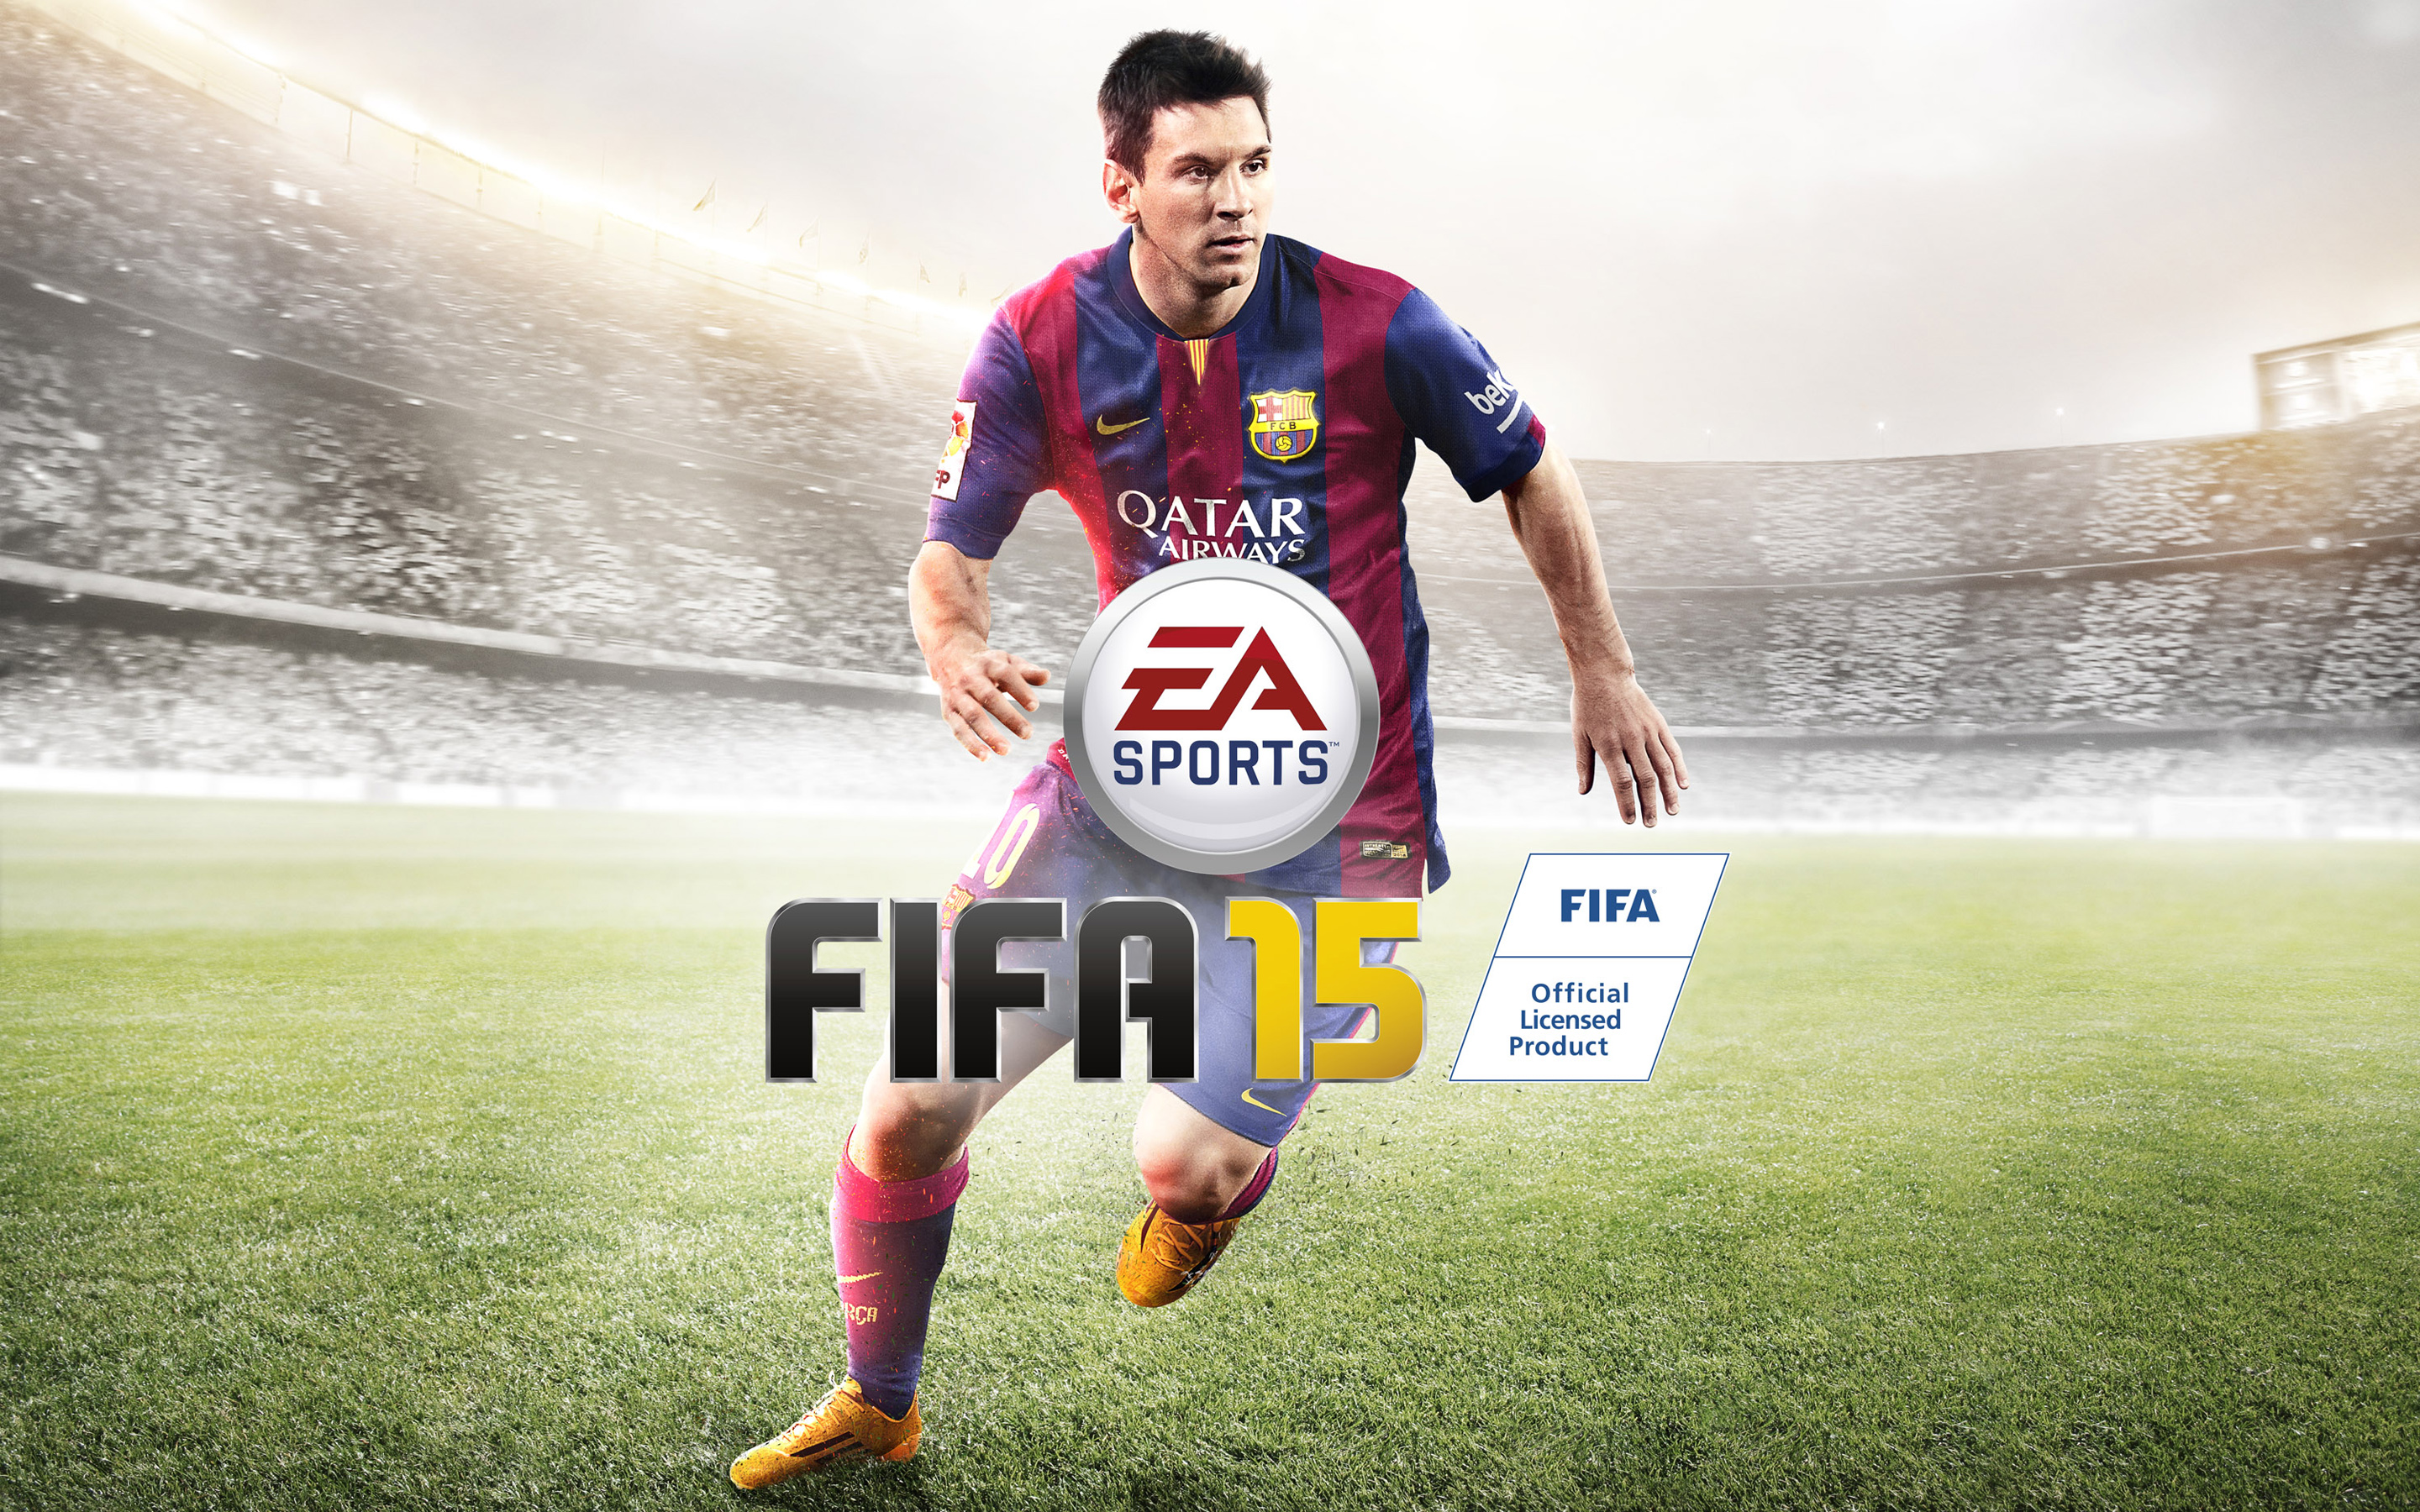
\includegraphics[width=7cm]{figuras/Fifa15}}
		}{
			\Fonte{\cite{fifa}}			
		}	
	\end{figure}

\section{Categoria de Jogos}
\label{sec:categoria-de-jogos}

É possível classificar os jogos em 3 categorias, sendo estas:
\begin{alineascomponto}

\item Jogos 2D\\
Implementados a partir de gráficos bidimensionais somente com uma camada.

 Perspectiva \textit{ Top-down} - tem a perspectiva sobre a cabeça do personagem e este pode se movimentar em qualquer angulo.
 \textit{Side Scroling} - tem a perspectiva do lado do personagem onde este se move para direita ou esquerda, comum em jogos de plataforma. Na figura 7 é possível verificar a representação gráfica de um plano 2D (bidimensional). \cite{graf}

\end{alineascomponto}


\begin{figure}[h!]
		\centering
		\Caption{\label{fig:exemplo-}Representação gráfica de um plano bidimensional}	
		\UECEfig{}{
			\fbox{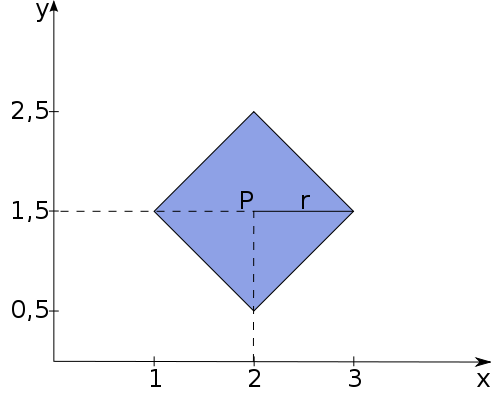
\includegraphics[width=7cm]{figuras/2D}}
		}{
			\Fonte{\cite{2d}}			
		}	
	\end{figure}

\begin{alineascomponto}
\pagebreak

\item Jogos 2.5D\\
Atribuído em jogos onde o 2D e o 3D são combinados para reproduzir um cenário mais realista. Nesta categoria os personagens são modelados em imagens 2D e se movimentam em um cenário 3D ou um personagem em 3D em um fundo 2D porém sendo mais comum um cenário que apresenta características de dimensão de profundidade a partir da sobreposição de imagens 2D.

Se divide na categorias: Isométrico, projeção oblíqua, \textit{billboarding} e escalamento do eixo Z. Na figura 8 é possível verificar a representação gráfica de um plano 2.5D (isométrico). \cite{graf}

\end{alineascomponto}

\begin{figure}[h!]
		\centering
		\Caption{\label{fig:exemplo-4}Representação gráfica de um espaço isométrico (2.5D)}	
		\UECEfig{}{
			\fbox{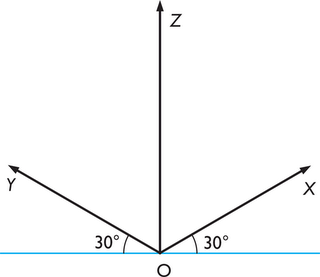
\includegraphics[width=7cm]{figuras/isometrico}}
		}{
			\Fonte{\cite{25d}}			
		}	
	\end{figure}
	\pagebreak
\begin{alineascomponto}

\item Jogos 3D\\
São jogos onde o cenário é modelado tridimensionalmente sendo possível o personagem mover-se em qualquer direção.
Se dividem nas categorias
\begin{alineascomponto}
\item 3D Fixo - Jogo onde a câmera é fixa.
\item Primeira pessoa - Jogo onde a câmera está na posição na altura dos olhos do personagem.
\item Terceira pessoa - Jogo aonde câmera está próxima ao personagem, sempre o acompanhando. 
\end{alineascomponto}
Na figura 9 é possível verificar a representação gráfica de um plano 3D (tridimensional). \cite{graf}
\end{alineascomponto}

\begin{figure}[h!]
		\centering
		\Caption{\label{fig:exemplo-7}Representação gráfica de um espaço tridimensional}	
		\UECEfig{}{
			\fbox{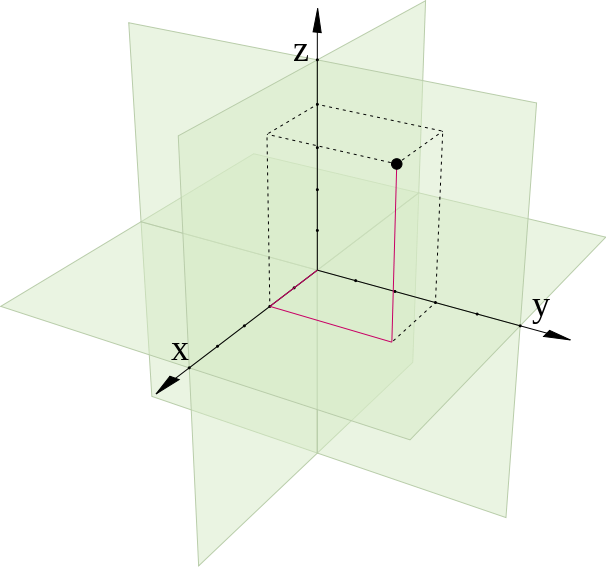
\includegraphics[width=7cm]{figuras/3D}}
		}{
			\Fonte{\cite{3d}}			
		}	
	\end{figure}
	
\begin{comment}

http://www.dca.fee.unicamp.br/~martino/disciplinas/ia369/trabalhos/t3g1.pdf
https://pt.wikipedia.org/wiki/G%C3%AAneros_de_jogos_eletr%C3%B4nicos
\end{comment}
\section{Engenharia de Software}
\label{sec:engenharia-de-software}

Sommerville  definiu engenharia de software como uma disciplina da engenharia que cuida de todos os aspectos da produção de software, desde a especificação do sistema até a sua manutenção, depois que ele entra em operação.

A engenharia é constituída de processos de software, que são conjuntos de atividades e resultados para se produzir um software. Existem quatro atividades fundamentais, são elas: 
\begin{alineascomponto}

\item Especificação de Software: o software a ser desenvolvido e as restrições para sua operação são definidos. 
Desenvolvimento de Software: o software deve ser feito atendendo suas especificações.
\item Validação de Software: o software tem de ser validado para garantir que está em cima do que o cliente deseja. 
\item Evolução do Software: o software sofre modificações para atender as necessidades do cliente. \cite{somm}
\end{alineascomponto}

No desenvolvimento de software, o principal objetivo é a criação de sistemas que atendam às necessidades dos clientes e usuários, ou seja, uma correta especificação dos requisitos se torna essencial para que o desenvolvimento tenha sucesso. Uma forma de entender melhor esses requisitos é dividindo-os em: Requisitos Funcionais e Requisitos Não-Funcionais. 


Os Requisitos Funcionais definem as funções que componentes do sistema ou sistemas devem executar. 
Os Requisitos Não-Funcionais incluem limitações no produto, como por exemplo: desempenho, confiabilidade, segurança e limitações no desenvolvimento, como custos e tempo, componentes a serem reutilizados, entre outros. \cite{vac}

\section{Desenvolvimento Mobile}
\label{sec:desenvolvimento-mobile}

Um dispositivo móvel pode ser definido como um computador de bolso, normalmente composto de uma tela e um teclado em miniatura podendo estes serem combinados em um só dispositivo conhecido como \textit{ touchscreen}.

Características dos dispositivos móveis:

\begin{alineascomponto}
 
\item Pequeno em tamanho
\item Baixo consumo de energia
\item Curto tempo de inicialização
\item Armazenamento de dados local e/ou remoto

	\end{alineascomponto}


Os dispositivos móveis mais populares são:

\begin{alineascomponto}
 
\item \textit{Smartphone}
\item \textit {Tablet}
\item Console portátil
\item \textit {Notebook}

	\end{alineascomponto}
	\cite{mov}
	\begin{comment} 
	http://www.dca.fee.unicamp.br/~martino/disciplinas/ia369/trabalhos/t1g1.pdf

https://books.google.com.br/books?id=pWc3AgAAQBAJ&pg=PA46&lpg=PA46&dq=estilo+de+jogos+digitais&source=bl&ots=P8i8N4DcJL&sig=uj-5ewjDs8v_Ea5XAtmdELqSQMY&hl=pt-BR&sa=X&ved=0ahUKEwj85cSisLvJAhWON5AKHXH-CAEQ6AEIWDAJ#v=onepage&q=estilo%20de%20jogos%20digitais&f=false
\end{comment}

A tecnologia que torna viável a existência dos dispositivos móveis começou a partir do primeiro celular inventado, em 3 de abril de 1983, o Motorola DynaTAC 8000x. Foi então que em 1992 a empresa Apple lançou no mercado o primeiro PDA que continha memória de 1MB e tela sensível ao toque, desde então esta tecnologia tem se desenvolvido e mostrado como vantagem  a possibilidade dos dados serem acessados em qualquer lugar a qualquer hora. \cite{1cel}

Dentre os dispositivos móveis citados, o que mais se destacam são os \textit{smartphones}. Um \textit{smartphone} (telefone inteligente) poder ser definido como um celular que possui muitas funções. Essas funções são realizadas de maneira mais eficientes do que um celular normal, em geral possuem internet wiFi, navegadores, é possível realizar a instalação de aplicativos e possui um Sistema Operacional (SO). \cite{smar} 

Uma das grandes vantagens dos \textit{smartphones} é a capacidade de qualquer pessoa desenvolver um aplicativo para o aparelho pois, em geral, o SO é um software aberto, onde existe a flexibilidade da criação de aplicativos.

Um Sistema Operacional é um conjunto de programas responsável por alocar recursos do hardware fornecendo também uma interface para o usuário. Os sistemas operacionais para smartphones mais conhecidos atualmente são: iOS, Android, Windows Mobile e BlackBerry \cite{oqsmar}

Segundo uma pesquisa realizada pela Gartner, o sistema operacional mais vendido em 2015 (para \textit{smartphones}) foi o Android e em segundo o iOS, conforme pode ser visto na figura 10. \cite{gar}
\begin{figure}[h!]
		\centering
		\Caption{\label{fig:exemplo-1}Venda Mundial de Smartphones por Sistemas Operacionais}	
		\UECEfig{}{
			\fbox{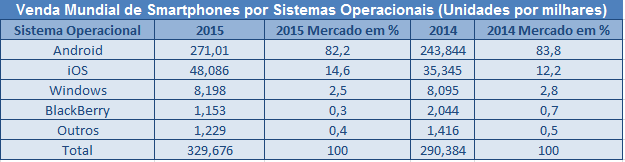
\includegraphics[width=13cm]{figuras/GartnetSamart}}
		}{
			\Fonte{Gartner, 2015}			
		}	
	\end{figure}

\subsection{Aplicativos Moveis}
Um aplicativo móvel, conhecido também como App é um software desenvolvido para dispositivos móveis, por exemplo, \textit{smartphones},  \textit{Tablets}, \textit{notebboks}, esses aplicativos podem ser nativos, Web ou híbridos. \cite{dif}

\begin{alineascomponto}

\item Aplicativos Nativos

São os aplicativos que podem ser acessados na tela principal através de seu ícone. Podem ser instalados através de um aplicativo de loja especifico para sua plataforma, como por exemplo o sistema iOS utiliza a App Store baixar seus aplicativos,enquanto o Android utiliza o Google Play. Esses aplicativo nativos residem no dispositivo.

\item \textit{Mobile Web Apps}

São aplicativos que na verdade são sites e não aplicativos raiz, como os nativos. São executados a partir de um navegador e normalmente criado um ícone na tela principal do dispositivo para que quando clicando ele acesse a URL determinada.

\item Aplicativos Híbridos

São os aplicativos que são parcialmente web e nativos.
Estes devem ser baixados pela loja de aplicativos, ficam armazenados no dispositivo porém podem também serem utilizado como web App.

	\end{alineascomponto} 
	
Segundo dados divulgados pelo Ministério de Ciência Tecnologia e Inovação (MCTI), o mercado de aplicativos móveis está em alta, movimentando mais de US\$ 25 bilhões por ano no Brasil, com expectativas de alcançar US\$ 70 milhões até 2017. \cite{mcti}
	
	
	\begin{comment}
http://www.luisaambros.com/blog/diferenca-entre-aplicativos-nativos-hibridos-e-mobile-web-apps/

http://www.correiobraziliense.com.br/app/noticia/tecnologia/2015/05/11/interna_tecnologia,482694/brasil-decola-na-industria-de-apps-e-mercado-acumula-lucros-nesta-deca.shtml
\end{comment}
	
\begin{comment}
http://www.telefonescelulares.com.br/o-que-e-smartphone/
http://pt.slideshare.net/cetorres/palestra-mobilidade-computao-mvel-dispositivos-e-aplicativos-2013
\end{comment}

\section{Android}
\label{sec:Android}
Android é um sistema operacional para dispositivos móveis, seu código é aberto (\textit{open-source}).Inicialmente desenvolvido pela Android Inc, em 2003 comprada pela empresa Google e desde 2007 mantida pela \textit{Open Handset Alliance} (OHA).

O sistema operacional Android possui seu núcleo (\textit{Kernel}) em Linux e utiliza Java como linguagem de programação padrão. Também utiliza de sua própria maquina virtual chamada de Dalvik.

A maquina virtual Dalvik possui grande diferença entre a Java Virtual Machine (JVM) o que faz seu desenho ser bem superior; a Dalvika é baseada em registradores e não em pilhas como a JVM.

A Dalvika executa seus arquivos na extensão ".dex" (Dalvik Executable) que nada mais são do que arquivos Java já previamente projetados e compilados realizando a otimização de memoria e compartilhamento de dados.

Na figura 11 é possível fazer um comparativo entre a JVM (.class) e a Dalvik VM (.dex). \cite{desa}

\pagebreak
\begin{figure}[h!]
		\centering
		\Caption{\label{fig:exemplo-2}Comparação do formato .class da JVM com o .dex usado pela Dalvik VM.}	
		\UECEfig{}{
			\fbox{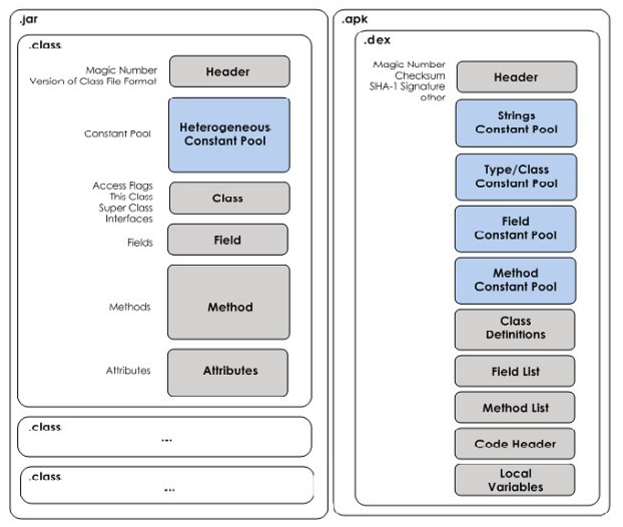
\includegraphics[width=13cm]{figuras/JvmDvm}}
		}{
			\Fonte{Marcelo Korjenioski, 2011}			
		}	
	\end{figure}

\subsection{Google Play }

Google Play também conhecida como Google Play Store é a loja virtual da Google para venda de aplicativos. Antigamente esta loja virtual recebia o nome de Android Market mas em 2002 seu nome mudou para haver a unificação de produtos.
No Google Play esta disponível para usuário baixar aplicativos gratuito e/ou pagos. \cite{gp}

\begin{comment}http://smartmundo.com/o-que-e-play-store/
\end{comment}
Para um desenvolvedor distribuir seus aplicativos na Google Play é necessario que o mesmo faça seu cadastro e pague uma quantia de U\$25,00, feito isso
sera possível fornecer seu aplicativo na loja virtual.
Um vez que o desenvolvedor tem a conta criada é possível ter acesso a comentários, estatísticas e erros de seus aplicativos. Caso o aplicativo seja pago, o lucro para o desenvolvedor é de 70\% do valor cobrado pelo aplicativo. \cite{tt}
\begin{comment}http://www.tutoriandroid.com/2012/05/como-publicar-no-google-play.html
\end{comment}

\subsection{Versões Disponíveis}

Desde de seu inicio, o Android nomeia suas versões com nomes de doces e sobremesas e segue uma ordem alfabética. Ainda não foi revelada pela empresa o real motivo deste padrão de nomenclatura.

Atualmente existem 13 versões do sistema operacional Android, estes apresentados na tabela 1. \cite{vs}

\begin{comment}
http://www.aplicativosandroid.com/conhecam-todas-as-versoes-do-android-e-seus-maravilhos-doces/3891 ---  e tabela ----- http://www.tecmundo.com.br/android/82344-linha-tempo-dentro-evolucao-do-sistema-android.htm
\end{comment}


\begin{table}[h!]
	\Caption{\label{tabela-android} Tabela contendo nome, versão e ano de lançamento dos sistemas Androids.}%
	\IBGEtab{}{%
		\begin{tabular}{ccc}
			\toprule
			Nome & Versões & Ano de Lançamento \\
			\midrule \midrule
			Alpha (Apple Pie)  & 1.0 & 2008 
			\\
			Beta (Banana Bread) & 1.1 & 2009 \\
			Cupcake & 1.5 & 2009\\
			Donut & 1.6 & 2009 \\
			Eclair & 2.0 e 2.1 & 2009 \\
			Froyo & 2.2 & 2010 \\
			Gingerbread & 2.3 & 2010 \\
			Honeycomb & 3.0; 3.1; 3.2 & 2011 \\
			Ice Cream Sandwich & 4.0 & 2011 \\
			Jelly Bean & 4.1; 4.2; 4.3 & 2012 e 2013 \\
			KitKat & 4.4 & 2013 e 2014 \\
			Lollipop & 5.0 & 2014 e 2015 \\
			Marshmallow & 6.0 & 2015 \\
			\bottomrule
		\end{tabular}%
	}{%
	\Fonte{\cite{doc}}%
}
\end{table}
\pagebreak
\section{Scrum}
\label{sec:scrum}

Scrum é uma metodologia ágil para gestão e planejamento de projetos de softwares e sua base fundamental pode ser bem descrita na figura 12.

	\begin{figure}[h!]
		\centering
		\Caption{\label{fig:exemplo}Prática do Scrum}	
		\UECEfig{}{
			\fbox{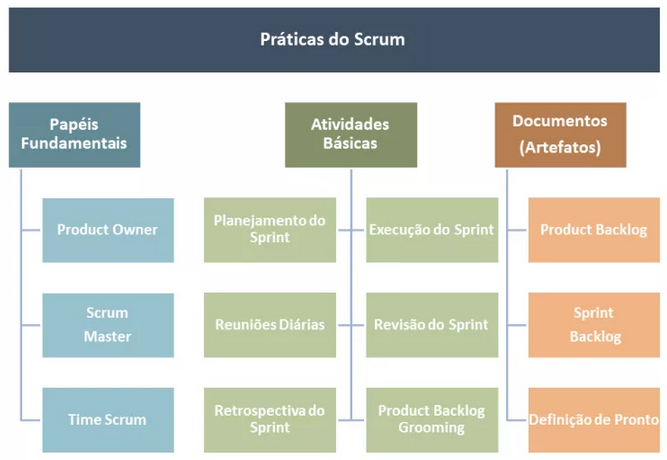
\includegraphics[width=10cm]{figuras/PraticaScrum}}
		}{
			\Fonte{\cite{scrum}}			
		}	
	\end{figure}

Cada equipe de Scrum, geralmente, possuem 3 papéis:
\begin{alineascomponto}
	\item \textit{Product Owner}
	
É responsável por decidir os recursos e funcionalidades utilizadas no projeto é também sua responsabilidade manter clareza no objetivo do projeto, para que haja uma melhor interação o ProductOwner geralmente colabora com o ScrumMaster.

	\item \textit{Scrum Master}
	
É de sua responsabilidade ajudar todos envolvidos a entender os valores, princípios e práticas do Scrum. Também fica responsável por melhorias no uso do Scrum e está sempre orientando para que não haja a perda de foco. 

	\item \textit{Development Team}
	
São todos da equipe responsáveis pelo desenvolvimento em si do software, possuem papéis como: arquiteto, testador, programador entre outros. Para esta equipe é recomendável que se organizem para determinar a melhor maneira de realizar o trabalho.
\pagebreak

	\end{alineascomponto}
	
		A figura 13 representa o processo de interação das atividades.


	\begin{figure}[h!]
		\centering
		\Caption{\label{fig:exemplo-3} Interação das atividades }	
		\UECEfig{}{
			\fbox{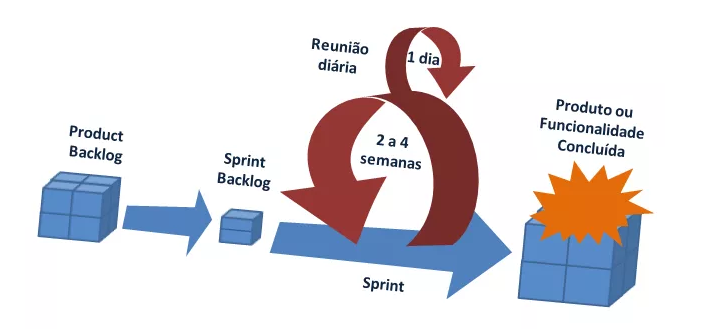
\includegraphics[width=10cm]{figuras/InteracaoScrum}}
		}{
		\Fonte{\cite{scrum}}			
	}	
	\end{figure}
	
O \textit{Product Owner} tem a visão final do produto, representado na figura 14 como grande cubo. Este cubo é "divido" em vários outros cubos pequenos, este chamado de \textit{Product Backlog}.

O \textit{Product Backlog} pode ser descrito, em uma forma simplificada, como pequenas etapas/objetivos para se chegar ao produto final.
Para planejar a prioridade dos \textit{Backloge} também quando e quanto tempo durará seu desenvolvimento, é utilizado o \textit{Sprint}.

O \textit{Sprint} tem duração mediana de 2 a 4 semanas, mas é também flexível dependendo do tempo desenvolvimento final estimado no começo do planejamento.

Também existe a técnica do \textit{Daily Scrum}, utilizado para o desenvolvimento deste jogo junto a sua monografia. Para o \textit{Daily Scrum}, é utilizado as três perguntas consideradas básicas para haver um melhor desenvolvimento de todos da equipe.
Estas são:

\begin{enumerate}
   \item O que fiz ontem que ajudou o time a atingir a meta do \textit{Sprint}?
   \item O que vou fazer hoje para ajudar o time a atingir a meta do \textit{Sprint}?
   \item  Existe algum impedimento que não permita a mim ou ao time atingir a meta do \textit{Sprint}?
 \end{enumerate}
 \cite{scrum}
 
Para a utilização do método Scrum há várias outras técnicas existentes, porém devido ao tempo curto e a quantidade de integrantes dispostos no desenvolvimento do jogo Caapora, foi somente utilizado os métodos acima.

\section{Controle de Versão}
\label{sec:Controle-de-Versão}

O controle de versão tem como objetivo a gerencia de versões de um mesmo projeto. Vários programadores podem trabalhar em um mesmo projeto sendo possível manter um histórico de atualizações.

Dentre as infinidades de vantagens para se utilizar um "controlador de versões" as três principais que se destacam são:
\begin{alineascomponto}
	
   \item Possibilidade de salvar o histórico
   \item Possibilidade de desenvolver versões diferentes
   \item Possibilidade de se programar em paralelo

	\end{alineascomponto}
	
	
O controle de versão funciona da seguinte forma: os históricos contendo as modificações de cada versão ficam armazenados em um repositório (servidor). Este processo dá à liberdade para que o desenvolvedor possa baixar a última versão, trabalhar em seu código e posteriormente atualizar a versão já previamente armazenada no servidor, este processo pode ser visto na figura 14.

	\begin{figure}[h!]
		\centering
		\Caption{\label{fig:exemplo-4} Funcionamento do Controle de Versão}	
		\UECEfig{}{
			\fbox{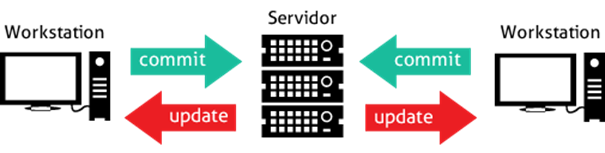
\includegraphics[width=13cm]{figuras/ControleVersao}}
		}{
		\Fonte{\cite{cv}}			
	}	
	\end{figure}
	
	Para que seja realizada a sincronização entre a \textit{workstation} e o servidor é necessário utilizar os comandos:
	
	\begin{alineascomponto}
\item \textit{Commit} - realiza o envio das alterações realizadas para o servidor gerando um novo histórico de atualizações.
\item \textit{Update} - realiza o envio da última versão contida no servidor para a \textit{workstation}.
\cite{cv}
	\end{alineascomponto}
	
	\subsection{Bitbucket}
	
No mercado atualmente existem dois grandes serviços que disponibilizam o controle de versionamento e estes são: Github e o Bitbucket.

O escolhido para desenvolvimento do Caapora games foi o Bitbucket, e é uma ferramente de domínio da empresa Atlassian e implementa dois padrões de versionamentos, o GIT e o Mercurial.


A equipe optou por utilizar este tipo de tecnologia para que houvesse uma melhor interação entre os membros e para que o desenvolvimento ocorresse simultaneamente e o
versionamento utilizado é o GIT. \cite{bit}

\section{Inteligência Artificial}
\label{sec:inteligencia-artificial}

A Inteligência Artificial (IA) é um ramo de pesquisa da ciência da computação que procura através de meio computacionais desenvolver mecanismos e/ou dispositivos que simulem a capacidade do ser humano de raciocinar e resolver problemas, ou seja, ser inteligente. 

O campo de IA tem como objetivo, o contínuo aumento da "inteligência"  do computador, pesquisando, para isto, os fenômenos da inteligência natural. Para este fim, IA é definida  como sendo uma coleção de técnicas suportadas por computador emulando algumas capacidades dos seres humanos. Esta coleção inclui:

\begin{alineascomponto}
	
   \item Resolução de problemas
   \item Compreensão de Linguagem Natural
   \item Visão e Robótica
   \item Sistemas Especialistas e Aquisição de Conhecimento
   \item Metodologias de Representação de Conhecimento

	\end{alineascomponto}
	
Hoje em dia a Inteligência Artificial é utilizada em vários fins, não só exclusivamente para informática e um dos pontos em que se destaca é para o desenvolvimento de jogos. 

Primeiramente utilizada em jogos clássicos como xadrez ou jogo da velha e atualmente utilizada para jogos digitais.


Os algoritmos de IA desenvolvidos para jogos digitais podem ser divididos em três blocos:

\begin{alineascomponto}
	
\item Movimento:

De como um personagem é movimentado, do local de inicial ate o destino final, também determina o cálculo do percurso, detectando objetos e desviando de obstáculos.
   
 \item Tomada de Decisão:
 
Cada personagem possui um conjunto de atividades e estados possíveis, estes sendo: estar parado, fugir, atacar adversário, entre outros. Para que cada ação seja possível, a personagem precisara fazer uma tomada de decisão analisando o contexto. Esta decisão pode ser de ativar um algoritmo de movimento, alterar um estado interno ou a animação. Não necessariamente essas alterações serão visuais.

\item Estratégia:

A maioria dos jogos digitais desenvolvidos com IA ocorrem nos dois tipos já citados estes também podem conter personagens que trabalham em grupo ou equipe contando com uma tomada de decisão individual.

	\end{alineascomponto}

	
As pesquisas iniciaram-se na Segunda Guerra Mundial com os cientistas Hebert Simon, Allen Newell,  Jonh McCarthy com o objetivo em comum de reproduzir uma maquina que simulasse o cérebro humano. \cite{ia}

\section{Busca Heurística}
\label{sec:Busca-Heurística}

A busca heurística pode ser definida como uma estratégia que faz uso do conhecimento específico do problema, sendo possível obter soluções mais eficientes do que uma estratégia sem informação. \cite{rus}

De acordo com \cite{el}, heurística é uma técnica eficiente para um processo de busca. A heurística, mesmo que as vezes possa passar por pontos de interesse despercebidos pode levar a direcionamentos interessantes. A heurística aprimora os caminhos a serem percorridos, entretanto pode desconsiderar o melhorar caminho a percorrer. 

Dentre as diversas heurísticas existentes, a que se destacou e mostrou melhor performance para o jogo Caapora foi o algoritmo A*
	

\subsection{Algoritmo A* (A estrela)}	
O A* (lê-se A estrela) é um algoritmo de busca de caminho \textit{(pathfinding)}. Segundo Russel (2003) A* é a forma mais eficiente pela busca da melhor escolha na qual avalia os nós combinando o custo para alcançar cada nó \textit{g(n)} e o custo do nó ate o objetivo h(n).

	\begin{equation}
		\begin{aligned}
		\textbf{ f(n) = g(n) + h(n)} 
		\end{aligned}
	\end{equation}
 
A função \textit{f(n)} representa o custo estimado da solução menos custosa passando por \textit{n} e chegando ao estado-objetivo. O A* utiliza também o método de lista aberta e fechada aonde listas abertas armazenam todos o nós que foram gerados porém ainda não examinados e a fechada armazena os nós que já analisados.

O algoritmo A* é completo e eficiente contanto que a função heurística \textit{f(n)} não superestime o custo ate o estado-objetivo.
\cite{aestar}
\begin{comment}
http://dsc.inf.furb.br/arquivos/tccs/monografias/2005-1jeanitabassanidasilvavf.pdf
file:///C:/Users/Talita/Downloads/601-1351-2-PB.pdf
\end{comment}

\section{Orientação Objeto}
\label{sec:orientação-objeto}	

O termo "Orientação a Objeto" conota o processo de modelar um sistema como "um grupo de agentes autônomos que colaboram para realizar algum procedimento de alto nível" (Booch, 1991:15)


\subsection{Classes e Objetos}	

Uma implementação de um objeto é definida por sua classe. A classe especifica os dados internos de um objeto, sua representação e define as operações que um ele pode realizar.
(Weinand, Gamma, Marty, 1988)


\subsection{Classes Abstratas}	

Classe abstrata é aquela que possui como propósito principal definir uma interface comum entre suas subclasses definindo parte ou toda a implementação de suas operações.
(Design Patterns: Elements of Reusable Object-Oriented Software (Weinand, Gamma, Marty, 1988, pg 27)


\subsection{Interface}	

Interface é a visão externa de, por exemplo, uma classe, objeto, componente, ou estrutura composta, que enfatiza sua abstração enquanto esconde sua estrutura e os segredos de seu comportamento.

Object-Oriented Analysis and Design with Applications Third Edition, Booch, 2007 pagina 596) 

\subsection{Padrões de Projeto}	
Christopher alexandre disse, "Cada Padrão descreve um problema que ocorre repetidamente no nosso ambiente, e então descreve a solução chave para o problema, de tal forma que você pode usar essa solução milhares de vezes, sem nunca vir a repeti-lo."

(A Pattern Language: Towns, Buildings, Construction Por Christopher Alexander,Sara Ishikawa,Murra, 1977, pg 12 )


\subsection{Singleton}	
Este Padrão de projeto garante que uma classe tenha apenas uma instância, e forneça um ponto global de acesso a ela.  
(Design Patterns: Elements of Reusable Object-Oriented Software - pagina 144)


\subsection{Object Pool}	
Este padrão de projeto segundo [Autor, Autor, ano ] gerencia o reuso de objetos quando eles consomem muito recurso para criar ou quando há um limite no numero de um tipo especifico de objetos que podem ser criados.

[Cap. 22 do livro Design Patterns Explained: A New Perspective on Object-Oriented Design, Alan Shalloway,James R. Trott ,  2004]
	\chapter{TECNOLOGIAS E FERRAMENTAS UTILIZADAS}
\label{cap:TECNOLOGIAS-E-FERRAMENTAS-UTILIZADAS}


\section{Unity 3D – Ambiente de Desenvolvimento}
\label{sec:Unity-3D-–-Ambiente-de-Desenvolvimento}

Unity é uma ferramenta com múltiplas utilidades na qual permite o usuário a desenvolver desde um jogo simples até de um de última geração.
Segundo o próprio site onde é fornecida a ferramenta "O Unity é um motor de desenvolvimento integrado que fornece uma funcionalidade pioneira para criação de jogos e outros conteúdos interativos. Poderá utilizar o Unity para montar sua arte e recursos em cenas e ambientes; adicionar física, editar e testar simultaneamente seu jogo e, quando preparado, publicar em suas plataformas escolhidas, tais como computadores fixos, a rede, iOS, Android, Wii, PS3 e Xbox 360." (Unity3D).
O Unity suporta três linguagens de programação que são Boo, JavaScript e o C\#, esta última sendo utilizada para desenvolvimento do jogo Caapora. O Unity também possui módulos que podem ser instalados possibilitando o desenvolvimento sem linha de código.


	\begin{figure}[h!]
		\centering
		\Caption{\label{fig:exemplo-1} Lorem ipsum dolor sit amet, consectetur adipiscing elit. Suspendisse commodo lectus et augue elementum varius.}	
		\UECEfig{}{
			\fbox{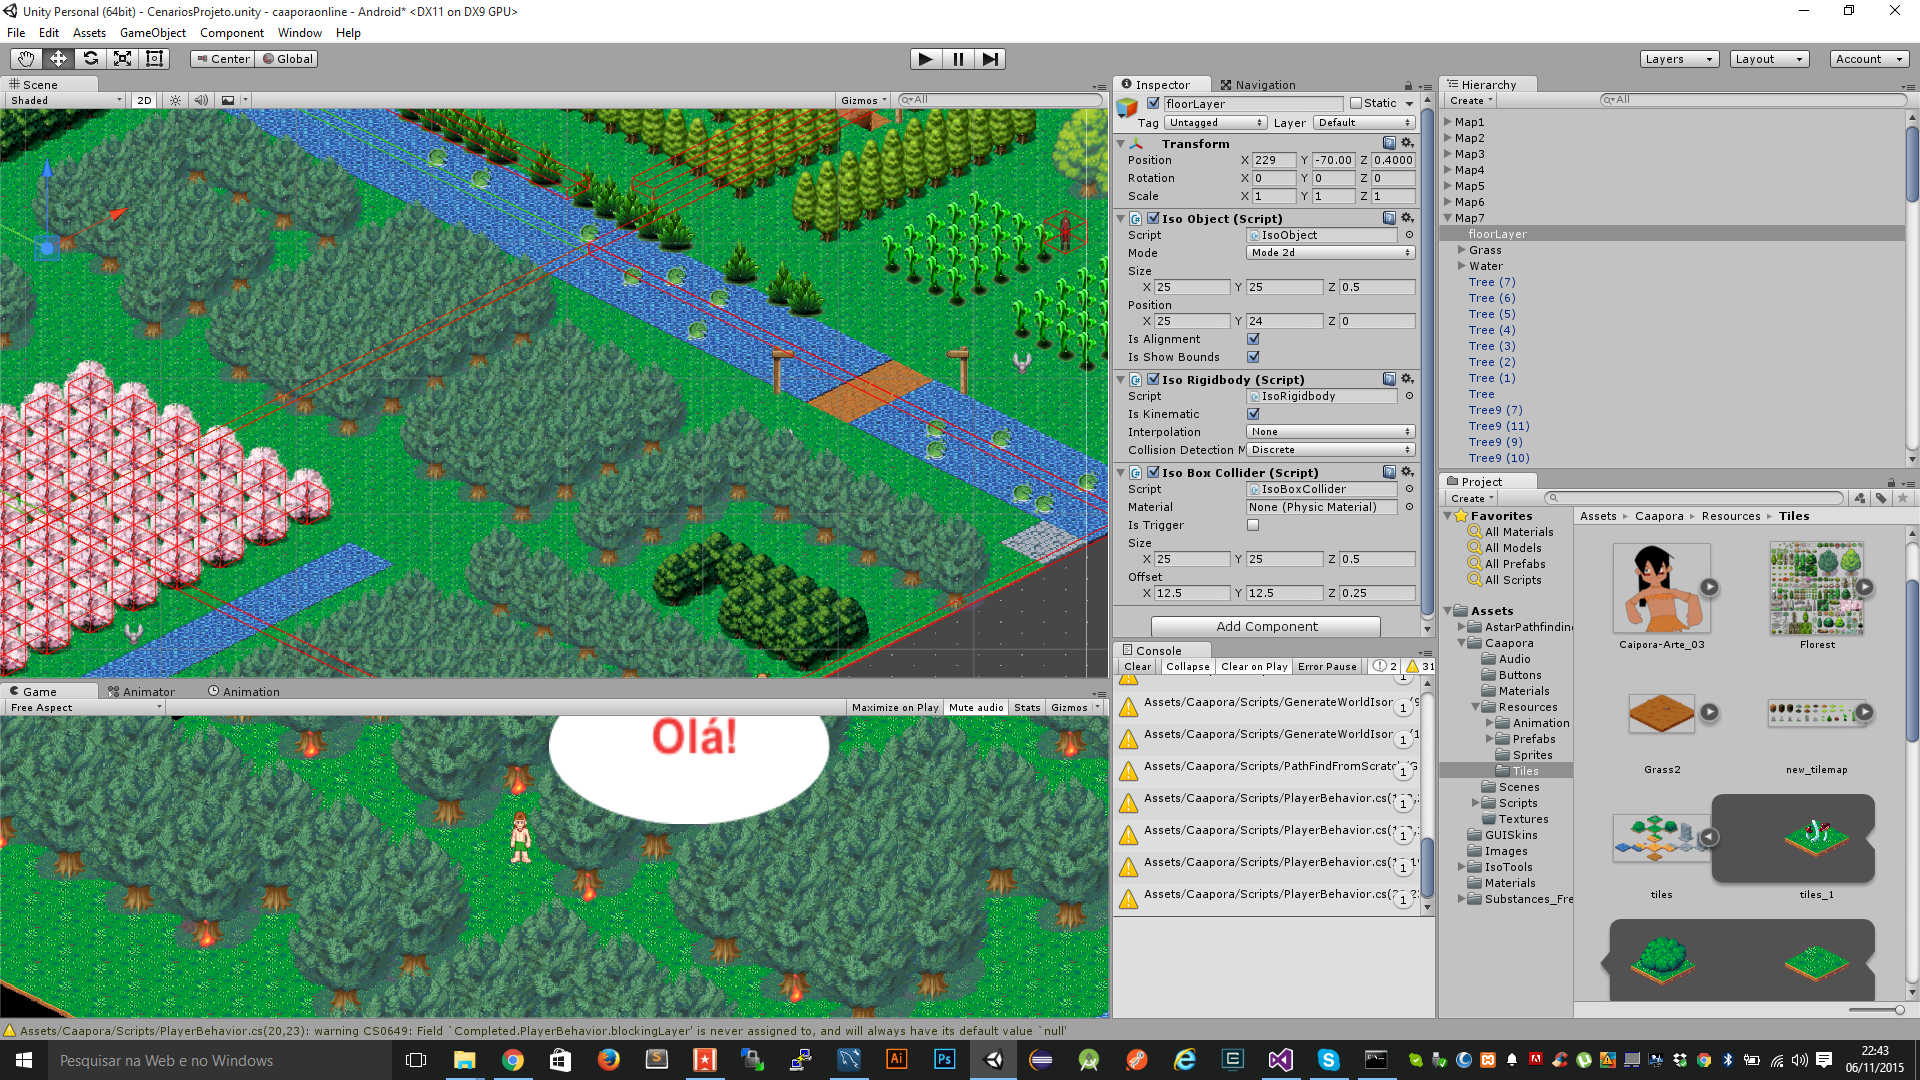
\includegraphics[width=13cm]{figuras/Unity}}
		}{
			\Fonte{Elaborado pelo autor}
		}	
	\end{figure}
	
Umas das principais vantagens de se utilizar o Unity é a possibilidade de desenvolver o jogo uma única vez e poder utiliza-lo em mais de 10 plataformas diferentes sem as necessidades de alterar o produto inicial. 
Algumas destas plataformas são: iPads, PC e iPhone

	
\section{Linguagem de programação Java Script}
\label{sec:Linguagem-de-programação-Java-Script}

JavaScript é uma linguagem para auxilio na criação de Home-Pages, as funções escritas em JavaScript podem ser embutidas dentro de seu documento HTML, possibilitando o incremento das funcionalidades do seu documento HTML com elementos interessantes. Sendo possivel: responder facilmente a eventos iniciados pelo usuário, incluir efeitos que tornem sua página dinâmica. Logo, podemos criar sofisticadas páginas com a ajuda desta linguagem. (GONÇALVES, 2005)

JavaScript é uma linguagem de programação criada por Brendan Eich em 1995, é uma linguagem dinâmica, orientada a objetos e possui similaridades com a linguagem C. 
É uma linguagem baseada em scripts e tem como sua principal característica em ser executado localmente, no lado do cliente, excluindo a necessidade de um servidor remoto.
Podemos dizer que JavaScript é mais uma extensão do HTML do que uma linguagem de programação propriamente dita. O primeiro browser a suportar JavaScript foi o Netscape Navigator 2.0 (GONÇALVES, 2005)

\section{Linguagem de programação C\#}
\label{sec:Linguagem-de-programação-Csharp}

C\# é uma linguagem elegante e de tipos protegidos, orientada a objeto e que permite aos desenvolvedores construírem uma variedade de aplicações seguras e robustas, compatíveis com o .NET Framework. É possível usar C\# para criar muito aplicativos de cliente do Windows, serviços Web XML, componentes distribuídos, aplicativos de cliente-servidor, aplicativos de banco de dados, e muito mais. O Visual C\# fornece um editor de códigos avançado, designers de interface de usuário convenientes, depurador integrado, e muitas outras ferramentas para facilitar o desenvolvimento de aplicativos baseados na linguagem C\# e no .NET Framework. (MICROSOFT, 2015)

A linguagem C\# foi desenvolvida pela Microsoft para ser um farmework .NET. 
O C\# é similar ao C++ e Java, sendo também uma linguagem fortemente tipada, orientada a objeto, portanto suporta heranças, polimorfismo e encapsulamento. 
Algumas características desta linguagem são: 

\begin{alineascomponto}
	\item Controle de versão: cada assembly gerado, seja como EXE ou DLL, tem informação sobre a versão do código. 

	\item Orientada a objetos: em C\#, qualquer variável tem de fazer parte de uma classe.  

	\item Linguagem gerenciada: todo gerenciamento de memória é feito pelo runtimevia GC (GarbageColletor), e não diretamente pelo programador, reduzindo assim as chances de cometer erros comuns.
\end{alineascomponto}

\section{Adobe Illustrato CC}
\label{sec:Adobe-Illustrato-CC}

A AdobeIllustrator CC é um software de gráficos vetoriais padrão do setor, usado em todo o mundo por designers de todos os tipos que querem criar gráficos digitais, ilustrações e tipografia para todos os tipos de mídia: impressão, web, interativa, vídeo e móvel. (Adobe, 2015)
O software Adobe Illustrator foi utilizado para a criação de sprites dos personagens e outras funcionalidades utilizadas no Capoora Games.

\begin{figure}[h!]
		\centering
		\Caption{\label{fig:exemplo-6} Lorem ipsum dolor sit amet, consectetur adipiscing elit. Suspendisse commodo lectus et augue elementum varius.}	
		\UECEfig{}{
			\fbox{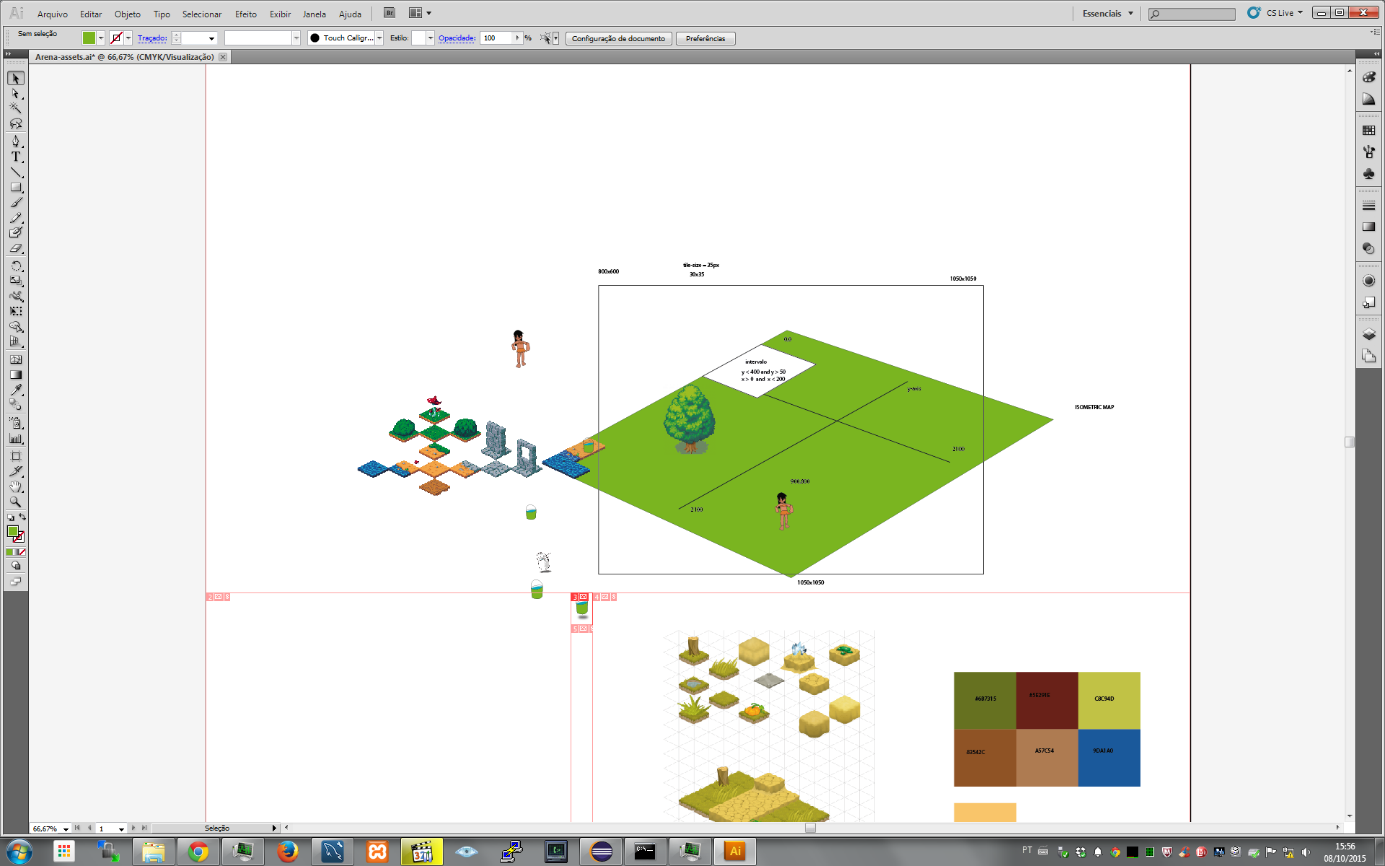
\includegraphics[width=13cm]{figuras/AdobeICC}}
		}{
			\Fonte{Elaborado pelo autor}
		}	
	\end{figure}
	
	\section{Visual Studio 2015}
\label{sec:Visual Studio 2015}

Visual Studio  é um ambiente de desenvolvimento da Microsoft na qual permite desenvolver aplicativo para plataformas WEB, Windows, Mac e Linux. É uma ferramenta direcionada para desenvolver em linguagem de programação C\# e o framework .NET.
Segundo o propio site da MICROSOFT, a empresa define a ferramenta como: " Um ambiente de desenvolvimento integrado e sofisticado para criação de aplicativos impressionantes para Windows, Android e iOS, de aplicativos Web modernos e serviços de nuvem."
Uma grande vantagem em se utilizar o Visual Studio 2015 é permitir o desenvolvimento em multiplataforma e também a disponibilidade de variadas extensões, de PHP a serviços de jogos.

\section{BitBucket}
\label{sec:BitBucket}

No mercado atualmente existem dois grandes serviços que disponibilizam o controle de versionamento e estes são: Github e o Bitbucket. O escolhido para desenvolvimento do Caapora games foi o Bitbucket, e é uma ferramente dedomínio da empresa Atlassian e implementa dois padrões de versionamentos, o GIT e o Mercurial.
 A equipe optou por utilizar este tipo de tecnologia para que houvesse uma melhor interação entre os membros e para que o desenvolvimento ocorresse simultaneamente e o versionamento utilizado é o GIT.

	
	\begin{quadro}[h!]	
		\centering
		\Caption{\label{qua:exemplo-1} Praesent ex velit, pulvinar at massa vel, fermentum dictum mauris. Ut feugiat accumsan augue}		
		\UECEqua{}{
			\begin{tabular}{|c|c|l|l|}
				\hline
				Quisque & pharetra & tempus & vulputate \\
				\hline
				E1 & Complete coverage by a single transcript & Both  & Complete\\
				\hline
				E2 & Complete coverage by more than & Both splice sites & Complete\\
				\hline
				E3 & Partial coverage & Both splice sites & Both \\				
				\hline
			\end{tabular}
		}{
			\Fonte{Elaborado pelo autor}
		}
	\end{quadro}
	
\lipsum[20]

	
	\begin{quadro}[h!]	
		\centering
		\Caption{\label{qua:exemplo-2} Duis faucibus, enim quis tincidunt pellentesque}		
		\UECEqua{}{
			\begin{tabular}{|c|c|}
				\hline
				Quisque & pharetra \\
				\hline
				E1 & Complete coverage by a single transcript \\
				\hline
				E2 & Complete coverage by more than \\
				\hline
				E3 & Partial coverage \\
				\hline
				E4 & Partial coverage \\
				\hline
				E5 & Partial coverage \\
				\hline
				E6 & Partial coverage \\
				\hline
				E7 & Partial coverage \\
				\hline
			\end{tabular}
		}{
			\Fonte{Elaborado pelo autor}
		}
	\end{quadro}

\lipsum[21]

Integer non lacinia magna. Aenean tempor lorem tellus, non sodales nisl commodo ut. Proin mattis placerat risus sit amet laoreet. Praesent sapien arcu, maximus ac fringilla efficitur, vulputate faucibus sem. Donec aliquet velit eros, sit amet elementum dolor pharetra eget. Integer eget mattis libero.
\Gls{ambiguidade}
\Gls{braile}
\Gls{coerencia}
\Gls{dialetos}
\Gls{elipse}
\Gls{locucao-adjetiva}
\Gls{modificadores}
\Gls{paronimos}
\Gls{sintese}
\Gls{borboleta}
	\chapter{Análise e Levantamento de Requisitos}
\label{chap:Analise-e-levantamento-de-requisitos}

\section{Análise de Produtos Semelhantes}
\label{sec:analise-de-produtos-semelhantes}

Um dos jogos que possui objetivos semelhantes ao do Caapora RPG e que coincidiu com a motivação do desenvolvimento é o jogo \textit{Pora: Free Cockatoos}

A\textit{Indonesian Society for Animal Welfare} (traduzido do inglês livre Sociedade Indonésio para o Bem Estar dos Animais)junto com outros desenvolvedores
criaram um aplicativo para conscientizar e educar em massa. “Muitas pessoas agora usam smartphones desde muito jovens”, diz Kinanti Kusumawardani, diretor executivo da \textit{Indonesian Society for Animal Welfare}. “Jogos para celular são um meio para chamar a atenção de maneira lúdica, uma vez que as pessoas parecem estar menos interessadas em ouvir palestras sobre o assunto”.

Para o desenvolvimento do jogo foi realizada uma competição em que os desenvolvedores deveriam criar um jogo que estimulasse a preservação da vida selvagem.

O Jogo \textit{Pora: Free Cockatoos} tem como personagem principal um peixe chamado Pora que possui um canhão onde ele lança torpedos aos caçadores que aprisionam as cacatuas.
Os vilões prendem as aves dentro de garrafas plasticas, uma pratica maldosa que realmente acontece.

“Os jogos podem fazer com que usuários se sintam envolvidos por uma causa sem que pareça algo muito sério”, afirmou Andi Surja Boediman, um parceiro da empresa que trabalha com os desenvolvedores. “É eficaz para promover a conscientização”. 

\begin{figure}[h!]
		\centering
		\Caption{\label{fig:exemplo-6} Jogo Pora: Free Cockatoos desenvolvido para conscientização dos mal tratos as aves da Indonésia}	
		\UECEfig{}{
			\fbox{
\includegraphics[width=9cm]{figuras/pora}}
		}{
			\Fonte{ANDA - Agencia de Noticias de Direitos Animais, 2015}
		}	
	\end{figure}
\pagebreak
\section{Requisitos do Sistema}
\label{sec:requisito-do-sistema}

\subsection {Requisitos Funcionais}

Foram definidos os seguintes requisitos funcionais, conforme exibido na Tabela 2:
\begin{table}[h!]	
	\centering
	\Caption{\label{tab:requiitos-funcionais}Requisitos Funcionais}	
	\IBGEtab{}{
		\begin{tabular}{cp{13cm}}
			\toprule
			Requisto & Função \\
			\midrule \midrule
			RF1 & O jogo deve ter um menu inicial contendo as seguintes opções: Iniciar Jogo e Opções. \\
			RF2 & Ao iniciar o jogo, o jogo deve apresentar um resumo sobre o cenário ao qual o jogador estará durante o jogo.\\
			RF3 & O jogo deve ter a opção de Pular o resumo do inicio do jogo.\\
			RF4 & A movimentação do personagem será controlada através do \textit{touchscreen} com controle direcional.\\
			R05 & Usuário terá a capacidade pegar o balde aguá quando tocado na tela do botão...\\
			RF6 & Usuário terá a capacidade jogar água no fogo apertando na tela o botão...\\
			RF7 & O jogo apresentará uma barra de vida do personagem Caapora que no qual ira diminuir toda vez que ele for 'queimado' \\
			RF8 & O balde devera ter uma barra de informação que mostrara o tanto de aguá que já foi enchido\\
			RF9 & Caso o usuário consiga apagar todo o fogo no tempo determinado, sera mostrada uma tela dizendo que o jogador conseguiu \\
			RF10 & Caso o usuário não consiga apagar todo o fogo em tempo determinado, sera mostrada uma tela dizendo que o jogador falhou\\
			
			\bottomrule
		\end{tabular}
	}{
	\Fonte{Elaborado pelo autor}
}
\end{table}

\subsection{Requisitos Não Funcionais}
Foram definidos os seguintes requisitos não funcionais, conforme exibido na Tabela 3:

\begin{table}[h!]	
	\centering
	\Caption{\label{tab:requisitos-nao-funcionais}Requisitos Não Funcionais}	
	\IBGEtab{}{
		\begin{tabular}{cp{13cm}}
			\toprule
			Requisito & Função \\
			\midrule \midrule
			RNF1 & O aplicativo deve funcionar na versão 3.0 do Android ou superior.\\
			RFN2 & O carregamento do jogo deve durar no máximo 10 segundos. \\
			RFN3 & A tela do dispositivo móvel deve ser \textit{touchscreen} e com tamanho minimo de XXX por XXXX\\
			
						\bottomrule
		\end{tabular}
	}{
	\Fonte{Elaborado pelo autor}
}
\end{table}

\section{Modelagem do Sistema}
\label{sec:modelagem-do-sistema}

A figura 19 apresenta o caso de uso do jogo, apresentando as ações que o jogador pode executar na aplicação.

\begin{figure}[h!]
		\centering
		\Caption{\label{fig:exemplo-} Caso de uso, ações do jogador}	
		\UECEfig{}{
			\fbox{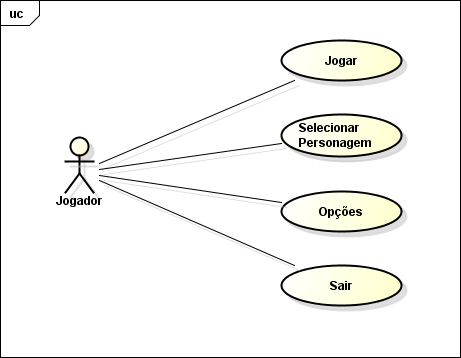
\includegraphics[width=13cm]{figuras/casodeuso}}
		}{
			\Fonte{Elaborado pelo autor}
		}	
	\end{figure}
\pagebreak


\begin{table}	
\centering
\Caption{\label{tab:caso-de-uso-jogar}Documentação do caso de uso Jogador}
\begin{tabular}{ | m{5cm} | m{8cm}| } 
\hline
\textbf {Nome do Caso de uso} & Jogar \\ 

\textbf {Ator Principal} & Jogador \\ 
\textbf {Resumo} & Esse caso de uso descreve as etapas percorridas por um jogador após ele selecionar a opção jogar \\
\textbf {Pré - condições} & Não se aplica\\
\hline
\textbf {Ações do Ator} & \textbf {Ações do Sistema}\\
\hline
1- O jogador seleciona a opção "Jogar" no menu principal. & 2 - Sistema exibe uma tela contendo uma mensagem informativa sobre o jogo.\\
3 - Jogador seleciona a opção "Pular" após ler as mensagens. & 4 - Sistema carrega o cenário do jogo.\\
\hline
\end{tabular}
\Fonte{Elaborado pelo autor}
\end{table}

\begin{table}	
\centering
\Caption{\label{tab:caso-selecionar-personagem}Documentação do caso de uso Selecionar Personagem}
\begin{tabular}{ | m{5cm} | m{8cm}| } 
\hline
\textbf {Nome do Caso de uso} & Selecionar Personagem \\ 

\textbf {Ator Principal} & Jogador \\ 
\textbf {Resumo} & Esse caso de uso descreve as etapas percorridas por um jogador durante a seleção de personagem \\
\textbf {Pré - condições} & Não se aplica\\
\hline
\textbf {Ações do Ator} & \textbf {Ações do Sistema}\\
\hline
1- O jogador seleciona a opção "Selecionar Personagem" na interface & 2 - Sistema exibe uma tela contendo personagens\\
3 - Jogador seleciona a personagem desejado & 4 - Sistema retorna para o menu principal.\\
\hline
\end{tabular}
\Fonte{Elaborado pelo autor}
\end{table}

\begin{table}	
\centering
\Caption{\label{tab:caso-de-uso-opcoes}Documentação do caso de uso Opções}
\begin{tabular}{ | m{5cm} | m{8cm}| } 
\hline
\textbf {Nome do Caso de uso} & Opções \\ 
\textbf {Ator Principal} & Jogador. \\ 
\textbf {Resumo} & Esse caso de uso descreve as etapas percorridas por um jogador após ele selecionar "Opções".\\
\textbf {Pré - condições} & Não se aplica.\\
\hline
\textbf {Ações do Ator} & \textbf {Ações do Sistema}\\
\hline
1- O jogador seleciona a opção "Opções" na interface & 2 - Sistema exibe uma tela contendo informações sobre áudio e vídeo.\\
3 - Jogador altera as configurações e salva & 4 - Sistema atualiza o jogo.\\
\hline
\end{tabular}
\Fonte{Elaborado pelo autor}
\end{table}

\begin{table}	
\centering
\Caption{\label{tab:caso-de-uso-sair}Documentação do caso de uso Sair}
\begin{tabular}{ | m{5cm} | m{8cm}| } 
\hline
\textbf {Nome do Caso de uso} & sair \\ 
\textbf {Ator Principal} & Jogador. \\ 
\textbf {Resumo} & Esse caso de uso descreve as etapas percorridas por um jogador após ele selecionar "Sair".\\
\textbf {Pré - condições} & Não se aplica.\\
\hline
\textbf {Ações do Ator} & \textbf {Ações do Sistema}\\
\hline
1- O jogador seleciona a opção "Sair" na interface & 2 - Sistema fecha o jogo..\\

\hline
\end{tabular}
\Fonte{Elaborado pelo autor}
\end{table}



\cite{Huetal2000} \lipsum[2] 

O autor \cite{lamport1986latex} e \cite{Maia2011} \lipsum[2] 







	
	\chapter{Desenvolvimento}
\label{cap:desenvolvimento}

Neste capitulo, serão apresentados os conceitos envolvidos no desenvolvimento do jogo.

\section{Cenas do jogo}
O jogo esta dividido em três cenas, que são: Menu Principal, Tutorial e Jogo.

\subsection{Menu Principal}
O menu principal é a primeira tela que o usuário terá contato ao abrir a aplicação. Nela o usuário poderá começar o jogo, selecionar personagem, alterar configuração de som e sair do jogo.

A figura 20 apresenta a tela inicial de jogo que será apresentada ao usuário.

\begin{figure}[h!]
		\centering
		\Caption{\label{fig:exemplo-1} Menu Principal}	
		\UECEfig{}{
			\fbox{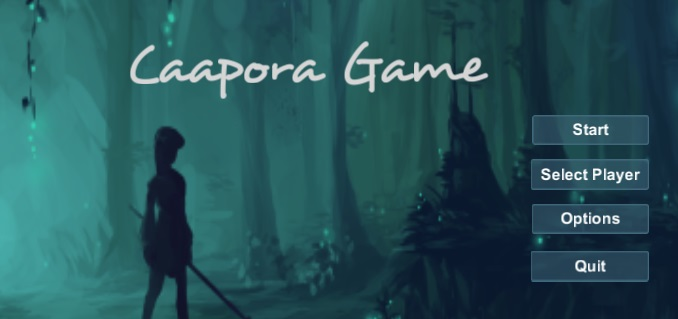
\includegraphics[width=13cm]{figuras/Menu}}
		}{
			\Fonte{Elaborado pelo autor}
		}	
	\end{figure}
	
\subsubsection{Botões}
Para criar os botões no menu foi utilizado um componente chamado UI, ele é um sistema que permite criar interfaces rápida e intuitivas. 

\subsubsection{Título }
Para criar o titulo foi usado um componente do sistema UI, chamado text que permite inserir um texto dentro de uma determinada área. Ele também permite editar alguns detalhes como tipo de fonte, tamanho e cor.

\subsubsection{Imagem de fundo}
Para inserir a imagem de fundo foi preciso adicionar um componente do UI chamado Panel. Ele delimita a área da do jogo, facilitando assim a inserção da imagem de fundo.

\subsection{Jogo}
A cena do jogo foi construída tendo como base o mapa isométrico, que é um cenário mais próximo do 3D. Foi utilizado alguns recursos como: \textit{Tilesets}, \textit{Sprites}, Animação, \textit{Collider} e \textit{Rigidbody}.

A figura 21 mostra o cenário completo.

\begin{figure}[h!]
		\centering
		\Caption{\label{fig:exemplo-1} Cenário do jogo Caapora RPG}	
		\UECEfig{}{
			\fbox{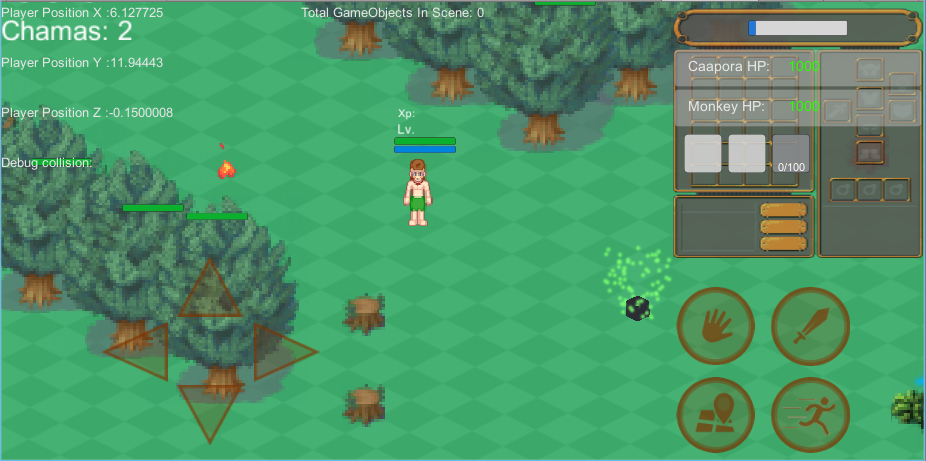
\includegraphics[width=13cm]{figuras/cena}}
		}{
			\Fonte{Elaborado pelo autor}
		}	
	\end{figure}

\subsubsection{Tilesets}
Os \textit{tilesets} são elementos gráficos dentro de uma imagem. Eles possuem tudo o que é preciso para a construção de mapas e são classificados de acordo ao tipo de mapa que será criado, no caso do jogo caipora, foi usado um \textit{tileset} da floresta.

Na figura 22 temos o \textit{tileset} usado no jogo.
\begin{figure}[h!]
		\centering
		\Caption{\label{fig:exemplo-1} Tileset utilizado na criação do cenário}	
		\UECEfig{}{
			\fbox{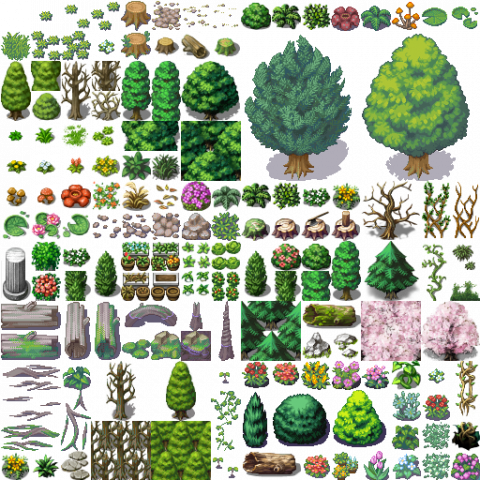
\includegraphics[width=8cm]{figuras/tileset}}
		}{
			\Fonte{\cite{tile}}
		}	
	\end{figure}

\subsubsection{Sprites}
Os \textit{sprites} são elementos gráficos dentro de uma única imagem que tem como objetivo criar animações. Eles foram usados na criação dos personagens e dos animais. 

A figura 23 mostra um dos \textit{sprites} do caipora.

\begin{figure}[h!]
		\centering
		\Caption{\label{fig:exemplo-1} Sprite do caipora correndo}	
		\UECEfig{}{
			\fbox{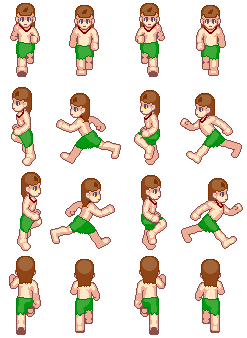
\includegraphics[width=6cm]{figuras/sprite}}
		}{
			\Fonte{Elaborado pelo autor}
		}	
	\end{figure}


\subsubsection{Animação}
A animação, tanto dos personagens quanto dos animais é criado dentro de um componente do Unity chamado Animation. Nele é criado um clipe de animação para cada ação do personagem, onde os \textit{sprites} são inseridos individualmente em uma linha do tempo e é determinada a velocidade que terá a animação.

A figura 24 mostra a criação do clipe de animação “Caapora-left”, onde temos uma sequencia de \textit{sprites} inseridos na linha do tempo.

\begin{figure}[h!]
		\centering
		\Caption{\label{fig:exemplo-1} Componente Animation}	
		\UECEfig{}{
			\fbox{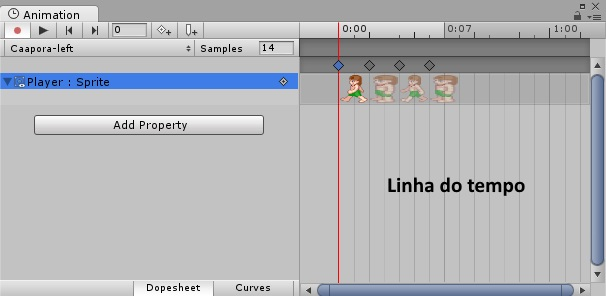
\includegraphics[width=13cm]{figuras/componente}}
		}{
			\Fonte{Elaborado pelo autor}
		}	
	\end{figure}


Após a criação dos clipes de animação, é necessário criar as transições entre eles. Para isso o Unity fornece um componente chamado \textit{Animator}. No \textit{animator}, conforme vemos na figura 25, os clipes de animação são ligados através das transições, que são as setas indo de um clipe para outro, e é criado condições para que haja a transição, ou seja, sempre que houver uma condição dentro do jogo, haverá uma mudança entre os clipes de animação.
	
\pagebreak

\begin{figure}[h!]
		\centering
		\Caption{\label{fig:exemplo-1} Componente Animator}	
		\UECEfig{}{
			\fbox{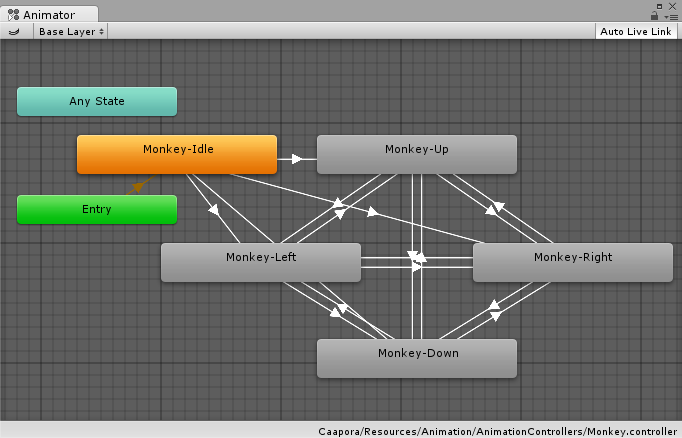
\includegraphics[width=10cm]{figuras/animator}}
		}{
			\Fonte{Elaborado pelo autor}
		}	
	\end{figure}


\subsubsection{Collider}
O colisor é um componente que impede que um objeto transpasse o outro, ele define a forma de um objeto para fins de colisões físicas.

Ele foi utilizado tanto nos personagens quantos nos objetos do cenário afim de evitar que esses objetos não atravessassem os demais.

Na figura 26 temos um tile e o elemento de colisão em volta. As linhas que traçam um retângulo representam o colisor.

	\begin{figure}[h!]
		\centering
		\Caption{\label{fig:exemplo-1} Elemento de colisão em volta de um tile}	
		\UECEfig{}{
			\fbox{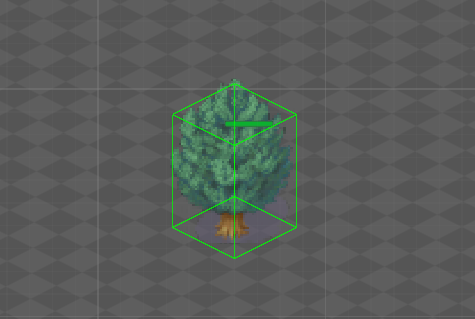
\includegraphics[width=10cm]{figuras/colisor}}
		}{
			\Fonte{Elaborado pelo autor}
		}	
	\end{figure}



\subsubsection{Rigidbody}
O \textit{Rigibody} é um componente que permite um comportamento físico em um determinado objeto. Quando esse componente é anexado ao objeto, automaticamente esse objeto vai responder a gravidade.

A figura 27 mostra o componente \textit{Rigidbody}.
	
	\begin{figure}[h!]
		\centering
		\Caption{\label{fig:exemplo-1} Componente Rigibody}	
		\UECEfig{}{
			\fbox{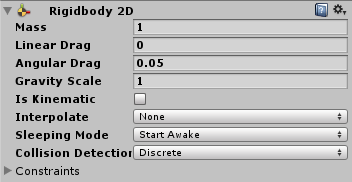
\includegraphics[width=10cm]{figuras/rigi}}
		}{
			\Fonte{Elaborado pelo autor}
		}	
	\end{figure}


\section{Mecanismos}

Nesta seção são apresentados os mecanismos principais que foram desenvolvidos dentro do jogo.

\subsection{Pegar Balde}

 Para implementar este mecanismo foram utilizados os componentes \textit{BoxCollider} do personagem e do elemento balde que ao identificar a colisão um com o outro, permite que o caipora pegue o balde inserindo-o em seu inventário retirando o objeto balde do cenário dando a impressão do objeto ter sido coletado.
 
 O estado do personagem então muda para um estado que identifica ele com o balde e da mesma forma, habilita a animação do caipora para a animação com o balde permitindo que ele colete a água. Na figura 28 é possível visualizar o personagem Caipora com o balde capturado.
 \pagebreak

\begin{figure}[h!]
		\centering
		\Caption{\label{fig:exemplo-1} Caipora com o balde}	
		\UECEfig{}{
			\fbox{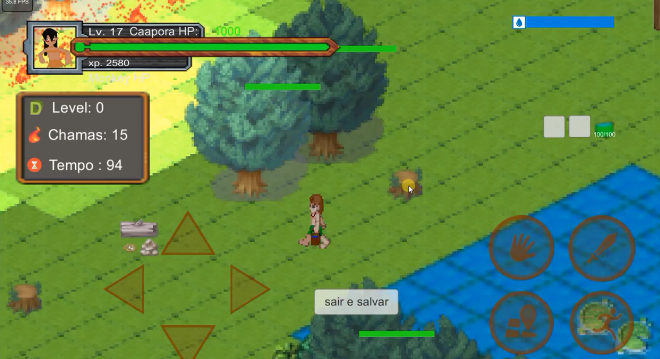
\includegraphics[width=10cm]{figuras/CaiporaComBalde}}
		}{
			\Fonte{Elaborado pelo autor}
		}	
	\end{figure}
	
	
\subsection{Encher o balde e Jogar Água}
Após o Caipora ter pegado o balde ele deverá enche-lo. Para encher o balde o personagem deve ter em seu inventário o balde e ao colidir com o objeto que representa a água um contador é incrementando e o painel de inventário da tela indica visualmente o nível de água que o balde encheu. 

De acordo com a quantidade de água disponível no balde o personagem então poderá lançar no cenário objetos do tipo borrifo de água, que se auto destrói, usando o método Destroy() e o recurso de \textit{Coroutines} do motor de jogos Unity3D, logo após ser lançado.

A figura 29 apresenta o Caipora jogando água nas chamas.

\begin{figure}[h!]
		\centering
		\Caption{\label{fig:exemplo-1} Caipora lançando água nas chamas}	
		\UECEfig{}{
			\fbox{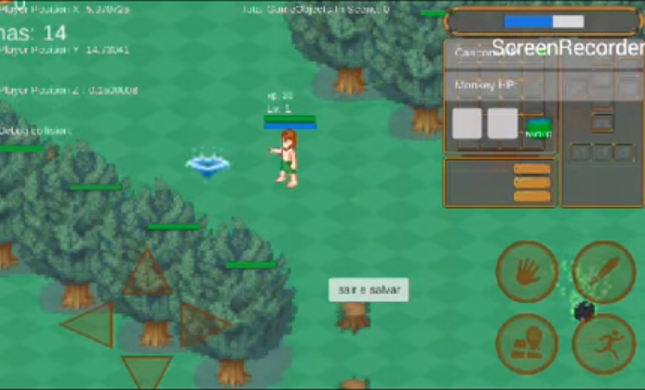
\includegraphics[width=9cm]{figuras/CaiporaJogandoAgua}}
		}{
			\Fonte{Elaborado pelo autor}
		}	
	\end{figure}
	
	
	
\subsection{Chamas}
São objetos que representam as chamas no mundo real e que causam destruição por onde passam, as chamas se multiplicam pelo cenário automaticamente, com o uso de \textit{Coroutines} do motor de jogos Unity3D,  em linha ou em círculos e conforme a dificuldade do jogo eles se espalham mais rapidamente. 

As chamas possuem pontos de danos na classe que as representa que são usados para reduzir os pontos de vida de qualquer personagens vivo no jogo, incluindo árvores. Este comportamento se encontra em todos os seres vivos do jogo que herdam a classe Creature. 

Para destruir este tipo de objetos é necessário que ele utilize o objeto do tipo borrifo de água, que é lançado pelo caipora, causando o efeito de ter apagado as chamas com a água borrifada.

A figura 30 apresenta as chamas se espalhando.

\begin{figure}[h!]
		\centering
		\Caption{\label{fig:exemplo-1} Fogo se alastrando}	
		\UECEfig{}{
			\fbox{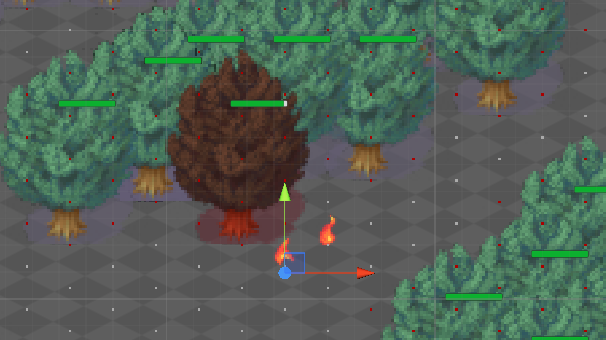
\includegraphics[width=10cm]{figuras/FogoSeAlastrando}}
		}{
			\Fonte{Elaborado pelo autor}
		}	
	\end{figure}
	
	
	
\subsection{Pathfinding}
O algoritmo de busca de melhor caminho (\textit{Pathfinding}) A* foi usado em duas situações no jogo; para personagens NPC (\textit{Non-Player Character}) amigos do personagem principal e para os inimigos que seguem o caipora e seus amigos com o objetivo de ataca-los.  Este recurso faz com que os personagens do jogo se movimentem sozinhos no mapa, melhorando consideravelmente a jogabilidade.


A figura 31 apresenta o personagem NPC \textit{Monkey} seguindo o Caipora com um caminho formado pelo algoritmo A*.

\begin{figure}[h!]
		\centering
		\Caption{\label{fig:exemplo-1} Exemplo de NPC}	
		\UECEfig{}{
			\fbox{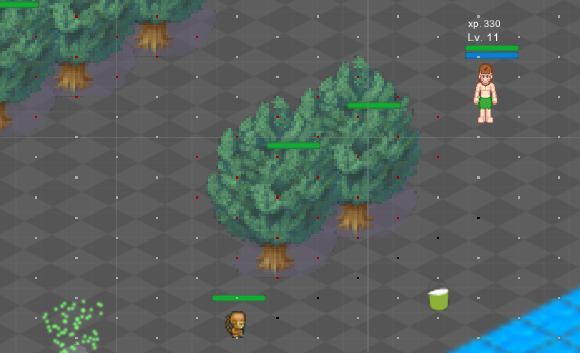
\includegraphics[width=10cm]{figuras/NPC}}
		}{
			\Fonte{Elaborado pelo autor}
		}	
	\end{figure}
	

	\section{Estrutura de Classes}
	A figura 32 apresenta a estrutura de Classes dos Personagens utilizada para o desenvolvimento do jogo.
	
	\begin{figure}[h!]
		\centering
		\Caption{\label{fig:exemplo-1} Estrutura de Classes de Personagens }	
		\UECEfig{}{
			\fbox{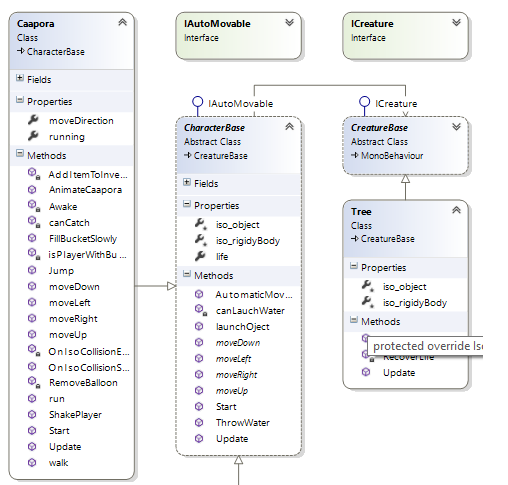
\includegraphics[width=15cm]{figuras/DiagramaClassesPersonagens}}
		}{
			\Fonte{Elaborado pelo autor}
		}	
	\end{figure}
	\pagebreak
	
\subsection{GameManager}
Está classe é responsável por gerenciador todo o ciclo de vida do jogo para isso ela  utiliza o padrão de projeto \textit{Singleton} que garante apenas uma instancia para um objeto durante toda a execução do jogo. Ela que implementa a maior parte da regra de negócio do jogo incluindo condições de vitórias e o fim de jogo.

\pagebreak

\subsection{Enemy}
Classe que representa os estados e comportamentos dos inimigos no jogo.

\subsection{NPC}
Personagens deste tipo implementam o algorítimo de \textit{pathfinding}  permitindo que movimentem-se sozinhos no jogo, possuindo uma inteligência artificial. Utiliza os métodos da classe \textit{Pathfinding} para personagens que perseguem o Caipora, é utilizando tanto amigos quanto em inimigos.

A figura 33 apresenta a estrutura de Classes dos NPCs utilizada para o desenvolvimento do jogo.

	\begin{figure}[h!]
		\centering
		\Caption{\label{fig:exemplo-1} Estrutura de Classes de NPC's }	
		\UECEfig{}{
			\fbox{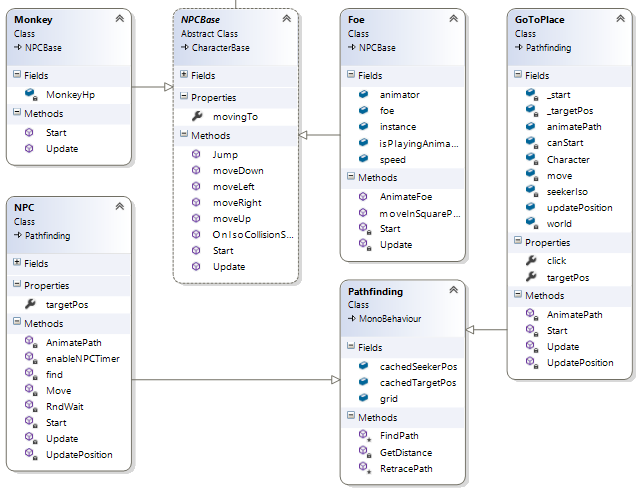
\includegraphics[width=15cm]{figuras/DiagramaClassesNpc}}
		}{
			\Fonte{Elaborado pelo autor}
		}	
	\end{figure}

\subsection{Inventory}
Esta classe tem por finalidade armazenar os objetos coletados pelo personagem principal e exibir suas características. Como exemplo temos o balde que no início do jogo o caipora tem que pegá-lo e enche-lo para apagar as chamas que estão queimando as árvores.


\subsection{Tree}
Esta classe representa as árvores no cenário e possui características herdadas da classe abstrata CreatureBase, possuindo assim pontos de vida e ataque podendo  morrer ao sofrer danos.


\subsection{Water}
Classe que representa a água no cenário, ao colidir com o fogo apaga-o. Ao colidir com o Caipora com o balde aumenta a quantidade de água no balde.


\subsection{Fire}
Classe que representa um fogo no \textit{game}, possui pontos de danos que são utilizados quando objetos do tipo seres vivos colidem com ele reduzindo seus pontos de vida.


\subsection{SpreadFire}
Classe que automatiza a expansão do fogo pelo cenário, extraindo as instâncias do \textit{Object Pool} e inserindo no mapa tanto em linha quanto em círculos.

\section{Funcionamento do jogo}
A aplicação do Caapora RPG se inicia no menu principal, onde o jogador pode iniciar o jogo, escolher um personagem, alterar configurações e sair do jogo como mostra a figura 34.

\pagebreak
\begin{figure}[h!]
		\centering
		\Caption{\label{fig:exemplo-1} Menu Principal}	
		\UECEfig{}{
			\fbox{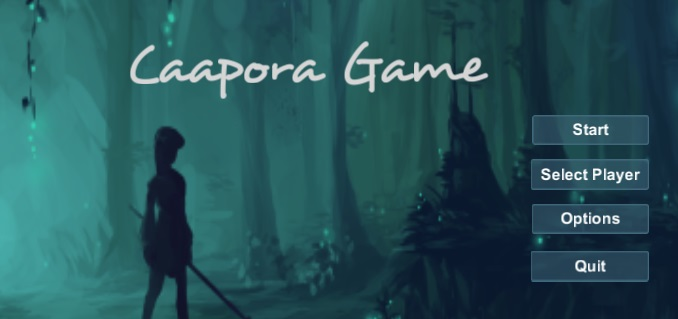
\includegraphics[width=13cm]{figuras/Menu}}
		}{
			\Fonte{Elaborado pelo autor}
		}	
	\end{figure}

Jogar: Ao selecionar a opção jogar, é apresentado ao jogador a tela do tutorial, onde terá uma breve descrição do que o jogador deverá fazer durante o jogo.

Personagem: Ao selecionar a opção personagem, o jogador será direcionado para tela onde ele poderá selecionar o Caipora ou o Curupira para jogar.

Opções: Ao selecionar o botão opções, o jogador poderá alterar algumas configurações como tirar a musica de fundo.

Sair: Ao selecionar o botão sair o jogador fecha o jogo.

Ao iniciar o jogo, a missão do jogador é apagar o fogo que está destruindo a mata, para isso ele deverá pegar um balde que está próximo ao rio, como mostra a figura 35.

\pagebreak
\begin{figure}[h!]
		\centering
		\Caption{\label{fig:exemplo-1} Jogador próximo ao balde.}	
		\UECEfig{}{
			\fbox{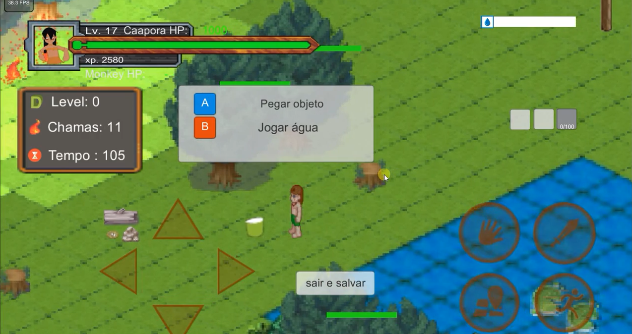
\includegraphics[width=13cm]{figuras/CaiporaPegandoBalde}}
		}{
			\Fonte{Elaborado pelo autor}
		}	
	\end{figure}

Ao pegar o balde o jogador deverá se dirigir até o rio, onde ao entrar em contato com o rio o balde encherá automaticamente. Na figura 36 temos o caipora enchendo o balde.

\begin{figure}[h!]
		\centering
		\Caption{\label{fig:exemplo-1} Jogador próximo ao rio.}	
		\UECEfig{}{
			\fbox{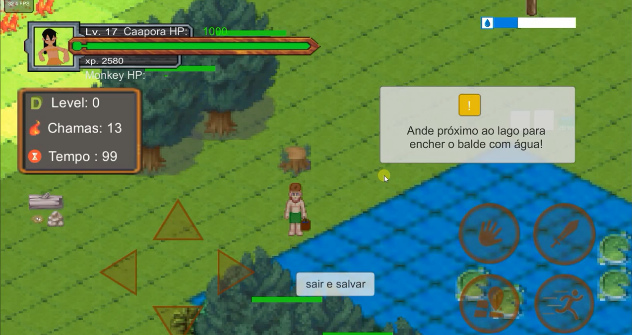
\includegraphics[width=13cm]{figuras/EnchendoBalde}}
		}{
			\Fonte{Elaborado pelo autor}
		}	
	\end{figure}

Com isso o jogador deverá procurar os lugares na floresta onde a mata esta em chamas. Dentro do jogo, o jogador terá um recurso que permitirá que ele visualize todo o mapa, sabendo assim onde se encontra o fogo. Na figura 37 temos o mapa completo do jogo.

\pagebreak
\begin{figure}[h!]
		\centering
		\Caption{\label{fig:exemplo-1} Mapa completo do jogo.}	
		\UECEfig{}{
			\fbox{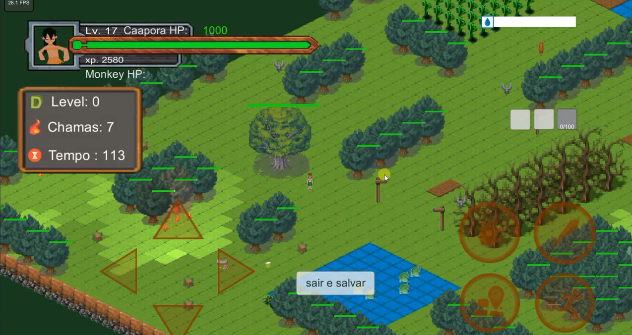
\includegraphics[width=13cm]{figuras/MapaCompleto}}
		}{
			\Fonte{Elaborado pelo autor}
		}	
	\end{figure}

Após localizar o local onde a mata esta pegando fogo, o jogador deverá lançar a água. A missão terminá quando todo o fogo na floresta for apagado. Os detalhes da missão estão descritos no \textit{Game Design Document} que esta no Apêndice.

	\chapter{Conclusão}
\label{chap:conclusoes-e-trabalhos-futuros}

Este projeto tem o objetivo de conscientizar as crianças sobre o desmatamento que ocorre em todo Brasil, principalmente na Floresta Amazônica. Para atingir esse objetivo, foi desenvolvido um jogo que é uma atividade rica em aprendizagem com o intuito de mostrar o que o país está enfrentando e o quanto isso é grave.

O jogo possui características importantes, já que o gênero (RPG com elementos de ação), faz com que o jogador assuma o personagem dentro do jogo, dando a ele uma perspectiva do que a natureza esta enfrentando.

Todo o desenvolvimento do jogo foi criado dentro do ambiente da Unity, isso devido à facilidade que o software oferece, como uma grande variedade de componentes que auxiliam na criação do jogo e também devido a ele ser multiplataforma, ou seja, apesar de ele ser para a plataforma Android, o jogo pode ser migrado para uma outra plataforma.

Com relação a performance, o jogo atingiu os requisitos de rodar à 30 quadros por segundo, visto que em jogos 2D onde são usados clipes de animação mais simples a taxa de 12 FPS é a mínima aceitável. 

Por fim, o projeto atendeu as expectativas visto que a principal mensagem que o jogo deveria transmitir foi alcançada, já que ele ilustra bem o que está ocorrendo na floresta, assim como também foi utilizado as tecnologias e ferramentas atuais.

\section{Trabalhos Futuros}
\label{sec:trabalhos-futuros}

Como trabalhos futuros a serem melhorados e implementados dentro do jogo, estima-se as seguintes funcionalidades:

\begin{alineascomponto}
	
   \item Criação de mais 3 cenários;
   \item Inclusão de mais animais;
   \item Criação do Curupira, que será o segundo personagem que o jogador poderá escolher;
   \item Melhoria do sistema de inteligência artificial utilizado no jogo, visando a realidade dos movimentos executados pelo IA;

	\end{alineascomponto}
	
	%Elementos pós-textuais	
	\bibliography{elementos-pos-textuais/referencias}
	\imprimirglossario	
	\imprimirapendices
		% Adicione aqui os apendices do seu trabalho
				\apendice{Game Design Document}
\label{ap:game-design-document}


\section {Introducao}
\label{ap:introducao}

Este documento visa informar aspectos conceituais e artísticos do jogo Caapora Game. O intuito do documento é estabelecer um objetivo comum para o desenvolvimento do jogo, auxiliando em duvidas gerais que possam aparecer nas fases de implementação do jogo em questão.

\subsection {Conceito}

Caapora game é um jogo 2D monojogador de ação habituada no cenário que será a floresta Amazônica, onde o jogador incorpora o Caipora e junto com a Vitória-Régia e o Boto cor-de-rosa precisa defender a floresta dos caçadores, lenhadores e mineradores.

\subsection {Gênero}
É um jogo no estilo ação em terceira pessoa, cujo cenário será em uma floresta.

\subsection {Publico Alvo}
O jogo destina-se a jogadores com faixa etária dos 5 aos 10 anos, pois se trata de um jogo infantil.

\subsection {Plataforma}
O jogo será desenvolvido dispositivos moveis, em especial \textit {smattphones}

\section {Historia e Narrativa}
\label{ap:historia-e-narrativa}

Descreve a historia do jogo, buscando informar onde se passa o jogo e os principais personagens envolvidos.

			

	

\end{document}